\documentclass[11pt,a4paper]{report}
\usepackage{graphicx}
\graphicspath{{./images/}}
\usepackage[utf8]{inputenc}
\usepackage{amsmath}
%\usepackage{tabto}
\usepackage{amsfonts}
\usepackage{amssymb}
\usepackage{tikz-cd}
\usepackage{amsthm}
\usepackage{xcolor}
\usepackage{tabularx}
\usepackage{booktabs}
\usepackage{algorithm}
%\usepackage{arevmath}
\usepackage[noend]{algpseudocode}
\usepackage[margin=1in]{geometry}

\usepackage[colorlinks=true,          % link colors, set to 'false' for print version
            linkcolor=blue,
            citecolor=red,
            urlcolor=blue]{hyperref}
            

%\setlength{\topmargin}{30mm}
%\addtolength{\topmargin}{-1in}
%\addtolength{\topmargin}{-\headsep}
%\addtolength{\topmargin}{-\headheight}
%\addtolength{\topmargin}{-\topskip}

%\setlength{\textheight}{270mm}
%\addtolength{\textheight}{\topskip}
%\addtolength{\textheight}{-\footskip}
%\addtolength{\textheight}{-30pt}

%\setlength{\oddsidemargin}{-1in}
%\addtolength{\oddsidemargin}{20mm}
%\setlength{\evensidemargin}{\oddsidemargin}

%\setlength{\textwidth}{170mm}

\newtheorem{defn}{Definition}[section]
 \newtheorem{thm}{Theorem}[section]
 \newtheorem{Lemma}{Lemma}[section]
 \newtheorem{Claim}{Claim}[section]
 \newtheorem{Prop}{Proposition}[section]
  \theoremstyle{definition}\newtheorem{Ex}{Example}[section]
 \newtheorem{Cor}{Corollary}[section]
 \newtheorem{claim}{Claim}[section]
 \newtheorem{conj}{Conjecture}  

\usepackage {amsfonts,amssymb}
%\usepackage{mathbbol}
\usepackage{latexsym}
\usepackage{mathrsfs}
\input xy
\xyoption{all}

\newcommand {\op}{\mathcal{O}\mathfrak{p}}
\newcommand {\Def}{\textrm{Def}}
\newcommand {\MC} {\textrm{MC}}
\newcommand {\Art}{\textrm{Art}_\CC}
\newcommand {\Kur}{\textrm{Kur}}
\newcommand {\LG} {^LG}
\newcommand{\fart}{\textrm{FArt}_\CC}
\newcommand{\fun}{\textrm{Fun}}
\newcommand{\sets}{\textrm{Sets}}
\newcommand{\tops}{\textrm{Top}}

\newcommand {\BB}{\mathbb{B}}
\newcommand {\CC}{\mathbb{C}}
\newcommand {\FF}{\mathbb{F}}
\newcommand {\KK}{\mathbb{K}}
\newcommand {\MM}{\mathbb{M}}
\newcommand{\NN}{\mathbb{N}}
\newcommand {\PP}{\mathbb{P}}
\newcommand{\QQ}{\mathbb{Q}}
\newcommand {\RR}{\mathbb{R}}
\newcommand {\SSS}{\mathbb{S}}
\newcommand {\VV}{\mathbb{V}}
\newcommand {\HH}{\mathbb{H}}
\newcommand {\WW}{\mathbb{W}}
\newcommand{\YY}{\mathbb{Y}}
\newcommand{\ZZ}{\mathbb{Z}}


\newcommand {\bal}{\boldsymbol{\alpha}}
\newcommand {\bbe}{\boldsymbol{\beta}}
\newcommand {\bga}{\boldsymbol{\gamma}}
\newcommand {\bmu}{\boldsymbol{\mu}}
\newcommand {\bom}{\boldsymbol{\omega}}
\newcommand {\bth}{\boldsymbol{\theta}}
\newcommand {\bph}{\boldsymbol{\phi}}
\newcommand {\bdh}{\boldsymbol{h}}
\newcommand {\bdk}{\boldsymbol{k}}
\newcommand {\bdE}{\boldsymbol{E}}
\newcommand {\bdU}{\boldsymbol{U}}
\newcommand {\bdP}{\boldsymbol{P}}
\newcommand {\ba}{{\bf a}}
\newcommand {\bb}{{\bf b}}
\newcommand {\bc}{{\bf c}}
\newcommand {\bd}{{\bf d}}
\newcommand {\bg}{{\bf g}}
\newcommand {\be}{{\bf e}}
\newcommand {\bdf}{{\bf f}}
\newcommand {\bp}{{\bf p}}
\newcommand {\bq}{{\bf q}}
\newcommand {\bv}{{\bf v}}
\newcommand {\bh}{{\bf h}}
\newcommand {\bk}{{\bf k}}
\newcommand {\br}{{\bf r}}
\newcommand {\bdu}{{\bf u}}
\newcommand {\bdv}{{\bf v}}
\newcommand {\bi}{{\bf i}}
\newcommand {\bj}{{\bf j}}
\newcommand {\bn}{{\bf n}}
\newcommand {\bs}{{\bf s}}
\newcommand {\bt}{{\bf t}}
\newcommand {\bu}{{\bf u}}
\newcommand {\bw}{{\bf w}}
\newcommand {\bx}{{\bf x}}
\newcommand{\by}{{\bf y}}
\newcommand {\bz}{{\bf z}}
\newcommand {\bB}{{\bf B}}
\newcommand{\bD}{{\bf D}}
\newcommand {\bE}{{\bf E}}
\newcommand {\bF}{{\bf F}}
\newcommand {\bG}{{\bf G}}
\newcommand {\bH}{{\bf H}}
\newcommand {\bK}{{\bf K}}
\newcommand {\bL}{{\bf L}}
\newcommand {\bM}{{\bf M}}
\newcommand {\bN}{{\bf N}}
\newcommand {\bO}{{\bf O}}
\newcommand {\bP}{{\bf P}}
\newcommand {\bQ}{{\bf Q}}
\newcommand {\bR}{{\bf R}}
\newcommand {\bT}{{\bf T}}
\newcommand {\bS}{{\bf S}}
\newcommand {\bU}{{\bf U}}
\newcommand {\bV}{{\bf V}}
\newcommand {\bW}{{\bf W}}
\newcommand {\bgamma}{\boldsymbol\gamma}
\newcommand {\bdelta}{\boldsymbol\delta}
\newcommand {\bDelta}{\boldsymbol\Delta}
%\newcommand{\qed}{{\ \bf qed}}

\newcommand {\rroot}{\mathbf{root}}
\newcommand {\coroot}{\mathbf{coroot}}
\newcommand {\weight}{\mathbf{weight}}
\newcommand {\coweight}{\mathbf{coweight}}
 \newcommand{\higgs}{\textrm{Higgs}}
\newcommand{\bun}{\textrm{Bun}}
\newcommand{\rk}{\textrm{rk}}
\newcommand{\ext}{\textrm{Ext}}
% \newcommand {\id}{\mathbb{1}}
% Use \id if using mathbbol instead of amssymb
\newcommand{\range}{\textrm{Range}}
\newcommand{\arccot}{\textrm{arccot}}

\newcommand{\thickslash}{\mathbin{\!\!\pmb{\fatslash}}}


\newcommand{\cA}{\mathcal{A}}
\newcommand{\cB}{\mathcal{B}}
\newcommand{\cC}{\mathcal{C}}
\newcommand{\cD}{\mathcal{D}}
\newcommand{\cE}{\mathcal{E}}
\newcommand{\cF}{\mathcal{F}}
\newcommand{\cG}{\mathcal{G}}
\newcommand{\cH}{\mathcal{H}}
\newcommand{\cI}{\mathcal{I}}
\newcommand{\cJ}{\mathcal{J}}
\newcommand{\cK}{\mathcal{K}}
\newcommand{\cL}{\mathcal{L}}
\newcommand {\cM}{\mathcal{M}}
\newcommand {\cN}{\mathcal{N}}
\newcommand {\cO}{\mathcal{O}}
\newcommand{\cP}{\mathcal{P}}
\newcommand{\cQ}{\mathcal{Q}}
\newcommand{\cR}{\mathcal{R}}
\newcommand{\cS}{\mathcal{S}}
\newcommand{\cT}{\mathcal{T}}
\newcommand{\cU}{\mathcal{U}}
\newcommand{\cV}{\mathcal{V}}
\newcommand{\cW}{\mathcal{W}}
\newcommand{\cX}{\mathcal{X}}
\newcommand{\cY}{\mathcal{Y}}
\newcommand{\cZ}{\mathcal{Z}}

\newcommand{\loc}{\mathcal{L}oc}
\newcommand{\Loc}{\textrm{Loc}}
\newcommand{\cih}{\mathpzc{h}}
\newcommand{\cx}{\mathpzc{x}}
\newcommand{\cy}{\mathpzc{y}}
\newcommand{\ce}{\mathpzc{e}}
\newcommand{\cf}{\mathpzc{f}}
\newcommand{\cl}{\mathpzc{l}}




 




\newcommand{\scA}{\mathscr{A}}
\newcommand{\scB}{\mathscr{B}}
\newcommand{\scC}{\mathscr{C}}
\newcommand{\scD}{\mathscr{D}}
\newcommand{\scE}{\mathscr{E}}
\newcommand{\scF}{\mathscr{F}}
\newcommand{\scG}{\mathscr{G}}
\newcommand{\scH}{\mathscr{H}}
\newcommand{\scI}{\mathscr{I}}
\newcommand{\scJ}{\mathscr{J}}
\newcommand{\scK}{\mathscr{K}}
\newcommand{\scL}{\mathscr{L}}
\newcommand{\scM}{\mathscr{M}}
\newcommand{\scP}{\mathscr{P}}
\newcommand{\scR}{\mathscr{R}}
\newcommand{\scO}{\mathscr{O}}
\newcommand{\scS}{\mathscr{S}}
\newcommand{\scT}{\mathscr{T}}
\newcommand{\scU}{\mathscr{U}}
\newcommand{\scV}{\mathscr{V}}
\newcommand{\scW}{\mathscr{W}}
\newcommand{\scX}{\mathscr{X}}
\newcommand{\scY}{\mathscr{Y}}
\newcommand{\scZ}{\scZ}

\newcommand{\uR}{\underline{\mathbb{R}}}
\newcommand {\uC}{\underline{\mathbb{C}}}


\newcommand{\fh}{\mathfrak{h}}
\newcommand{\fa}{\mathfrak{a}}
\newcommand{\fb}{\mathfrak{b}}
\newcommand{\fc}{\mathfrak{c}}
\newcommand{\fg}{\mathfrak{g}}
\newcommand{\fk}{\mathfrak{k}}
\newcommand{\fl}{\mathfrak{l}}
\newcommand{\fm}{\mathfrak{m}}
\newcommand{\fn}{\mathfrak{n}}
\newcommand{\fo}{\mathfrak{o}}
\newcommand{\fp}{\mathfrak{p}}
\newcommand{\fr}{\mathfrak{r}}
\newcommand{\fs}{\mathfrak{s}}
\newcommand{\fsu}{\mathfrak{su}}
\newcommand{\ft}{\mathfrak{t}}
\newcommand{\slt}{\mathfrak{sl}_2(\CC)}
\newcommand{\sln}{\mathfrak{sl}(n)}
\newcommand{\fsl}{\mathfrak{sl}}
\newcommand{\fu}{\mathfrak{u}}
\newcommand{\fv}{\mathfrak{v}}
\newcommand{\fx}{\mathfrak{x}}
\newcommand{\fy}{\mathfrak{y}}
\newcommand{\fz}{\mathfrak{z}}
\newcommand{\fA}{\mathfrak{A}}
\newcommand{\fB}{\mathfrak{B}}
\newcommand{\fD}{\mathfrak{D}}
\newcommand{\fM}{\mathfrak{M}}
\newcommand{\fR}{\mathfrak{R}}
\newcommand {\fU}{\mathfrak{U}}
\newcommand {\fV}{\mathfrak{V}}
\newcommand {\fW}{\mathfrak{W}}
\newcommand{\fX}{\mathfrak{X}}
\newcommand{\faff}{\mathfrak{aff}}

\newcommand{\Aff}{\textrm{Aff}}

\newcommand{\sym}{\textrm{Sym}}

\newcommand {\dbar}{\overline{\partial}}
\newcommand {\zbar}{\overline{z}}
\newcommand {\zvec}{\underline{z}}
\newcommand {\dzbar}{d\overline{z}}
\newcommand {\Nbar}{\overline{N}}
\newcommand {\Kbar}{\overline{K}}
\newcommand{\diff}{\textrm{Diff}}

%\newcommand {\hom}{\textrm{Hom}}

\newcommand{\mhom}{\textrm{Hom}}
\newcommand {\mend}{\textrm{End}}
\newcommand {\misom}{\textrm{Isom}}
\newcommand {\maut}{\textrm{Aut}}
\newcommand{\pr}{\textrm{pr}}

\newcommand {\sisom}{\underline{Isom}}
\newcommand {\saut}{\underline{Aut}}
\newcommand {\shom}{\textrm{\underline{Hom}}}
\newcommand {\send}{\underline{End} }

\newcommand{\dra}{M^{an}_{DR}(X,G)}
\newcommand{\dr}{M_{DR}(X,G)}

\newcommand {\ad}{\textrm{ad} }
\newcommand{\Ad}{\textrm{Ad}}

\newcommand{\lspan}{\textrm{span}}
\newcommand{\img}{\textrm{Im }}
\newcommand{\spec}{\textrm{Spec }}
\newcommand{\specan}{\textrm{Spec}^{an}}
\newcommand{\gspec}{\underline{\textrm{Spec }}}
\newcommand {\cok}{\textrm{coker}}
\newcommand{\tot}{\textrm{tot }}
\newcommand{\tildel}{\widetilde{\delta}}
\newcommand{\ctimes}{\otimes_\CC}
\newcommand{\sotimes}{\otimes_{\cO_X}}
\newcommand{\pic}{\textrm{Pic}}
\newcommand{\tr}{\textrm{tr }}

\newcommand  {\eps}{\varepsilon}
\newcommand {\kap}{\varkappa}
\newcommand {\io}{\iota}
\newcommand {\fii}{\varphi}

\newcommand{\Higgs}{{\bf Higgs}}
\newcommand{\Bun}{{\bf Bun}}
\newcommand{\gHiggs}{\op{\boldsymbol{\mathcal{H}iggs}}}
\newcommand{\Prym}{{\bf Prym}}
\newcommand{\Jac}{{\bf Jac}}
%\newcommand{\bh}{\boldsymbol{h}}
%\newcommand{\bH}{\boldsymbol{\mathcal{H}}}
\newcommand{\rts}{{\sf root}}
\newcommand{\wts}{{\sf weight}}
\newcommand{\crts}{{\sf coroot}}
\newcommand{\cwts}{{\sf coweight}}
\newcommand{\chr}{{\sf char}}
\newcommand{\cchr}{{\sf cochar}}

\newcommand{\Aut}{\textrm{Aut}}
\newcommand{\Der}{\textrm{Der}}
\newcommand{\spin}{\textrm{Spin}}
\newcommand{\spinc}{\textrm{Spin}^c}
%\newcommand{\U}{\boldsymbol{U(1)}}

\newcommand{\Mat}{\textrm{Mat}}

\newcommand{\hookr}{\hookrightarrow}

%%%%%%%%%%%%%%%%%%%%%%%%%%%%%%%%%%%%%%%%%%%%%%%%%%%%%%%%%%%%%%%%%%%%%%%%%
% Long exact sequence macro
%%%%%%%%%%%%%%%%%%%%%%%%%%%%%%%%%%%%%%%%%%%%%%%%%%%%%%%%%%%%%%%%%%%%%%%%%

\newcommand{\les}[9]{
\xymatrix{
 0 \ar[r] & {#1} \ar[r]  &  {#2} \ar[r]  &  {#3}
\ar@{->}`r/10pt[d] `[l] `^dl[dlll]  `^dr/10pt[dll]    [dll] \\
 &  {#4} \ar[r] & {#5} \ar[r] & {#6}
\ar@{->}`r/10pt[d] `[l] `^dl[dlll]  `^dr/10pt[dll]    [dll] \\
 & {#7} \ar[r]  & {#8} \ar[r] & {#9}
\ar@{->}`r/10pt[d] `[l] `^dl[dlll]  `^dr/10pt[dll]    [dll] \\
 & 0 \ar[r] & \cdots & }
}


%%%%%%%%%%%%%%%%%%%%%%%%%%%%%%%%%%%%%%%%%%%%%%%%%%%%%%%%%%%%%%%%%%%%%%%%%

\newcommand{\lestwo}[9]{
\xymatrix{     
 0 \ar[r] & {#1} \ar[r]  &  {#2} \ar[r]  &  {#3} 
\ar@{->}`r/10pt[d] `[l] `^dl[dlll]  `^dr/10pt[dll]    [dll] \\
 &  {#4} \ar[r] & {#5} \ar[r] & {#6} 
\ar@{->}`r/10pt[d] `[l] `^dl[dlll]  `^dr/10pt[dll]    [dll] \\
 & {#7} \ar[r]  & {#8} \ar[r] & {#9} }
}

%%%%%%%%%%%%%%%%%%%%%%%%%%%%%%%%%%%%%%%%%%%%%%%%%%%%%%%%%%%%%%%%%%%%%%%%%
% Long exact sequence macro
%%%%%%%%%%%%%%%%%%%%%%%%%%%%%%%%%%%%%%%%%%%%%%%%%%%%%%%%%%%%%%%%%%%%%%%%%

\newcommand{\lesthree}[5]{
\xymatrix{     
 0 \ar[r] & {#1} \ar[r]  &  {#2} \ar[r]  &  {#3} 
\ar@{->}`r/10pt[d] `[l] `^dl[dlll]  `^dr/10pt[dll]    [dll] \\
 &  {#4} \ar[r] & {#5} & }
}


%%%%%%%%%%%%%%%%%%%%%%%%%%%%%%%%%%%%%%%%%%%%%%%%%%%%%%%%%%%%%%%%%%%%%%%%%
% Long exact sequence macro
%%%%%%%%%%%%%%%%%%%%%%%%%%%%%%%%%%%%%%%%%%%%%%%%%%%%%%%%%%%%%%%%%%%%%%%%%

\newcommand{\lesfour}[8]{
\xymatrix{     
 0 \ar[r] & {#1} \ar[r]  &  {#2} \ar[r]  &  {#3} 
\ar@{->}`r/10pt[d] `[l] `^dl[dlll]  `^dr/10pt[dll]    [dll] \\
 &  {#4} \ar[r]^-{#8} & {#5} \ar[r] & {#6} 
\ar@{->}`r/10pt[d] `[l] `^dl[dlll]  `^dr/10pt[dll]    [dll] \\
 & {#7} \ar[r]  & \cdots  &  }
}

\newcommand{\equivclass}[1]{%
  #1/{\sim}%
}
\newcommand{\equivcls}[1]{%
  #1/\!{\sim}%
}

%


\include{biblio}

\title{Optimization over Grassmann Manifolds}
\author{Author: Milos Vukadinovic}
\date{\parbox{\linewidth}{\centering%
  \endgraf\bigskip
  Advisor: Peter Dalakov \endgraf\medskip
  \bigskip
  Department\ of Mathematics,  \endgraf
  American University in Bulgaria \endgraf
  \bigskip
  \today}}
%\input{preamble}
\begin{document}
\maketitle

\begin{abstract}
We present optimization methods for functions whose domain lies on Grassmann manifold.
Such functions are ubiquitous because data with subspace-structured features, orthogonality, or low-rank constraints is naturally expressed using Grassmann manifold.
We consider two different representations of the Grassmann manifold: a quotient of the Stiefel manifold and a set of projectors.
We then develop Grassmannian gradient descent and Grassmannian Newton method on these representations.
We demonstrate the efficiency of Grassmannian algorithms by optimizing Rayleigh quotient and conclude that our algorithms converge faster,
generalize better and perform as well as the best-known problem-specific algorithms. 
\end{abstract}

\setcounter{tocdepth}{1}
\tableofcontents






\chapter{Introduction}
Constrained optimization is the process of optimizing an objective function with respect to some variables with the presence of constraints on those variables.
In our paper, we consider geometric constraints, which express that the solution to the optimization problem lies on a manifold.
Specifically, we consider problems where the solution lies on the Grassmann manifold - $G(p, n)$ a set of $p$ dimensional subspaces in a higher $n$-dimensional space.
Such problems are ubiquitous because data with subspace-structured features, orthogonality constraints, or low-rank constraints can be naturally expressed using the Grassmann manifold.
For example, symmetric eigenvalue problems, nonlinear eigenvalue problems, electronic structure computations, and signal processing can all be optimized over $G(p, n)$.
In our paper, we first show how the Grassmann manifold can be considered as a quotient manifold and as a set of projectors.
Then, we develop Gradient Descent and Newton’s algorithm on the Grassmann manifold and study its applications to eigenvalue and eigenvector computations.
\par
A framework for algorithms involving these constraints was first introduced by Edelman et al \cite{edelman_geometry_1998} .
They used a quotient manifold representation to develop the Newton algorithm, which inspired a line of works that improve the algorithm or find a different application \cite{hamm_grassmann_nodate} \cite{ma_flag_2020} \cite{johnsson_optimization_nodate} \cite{tripuraneni_averaging_2018}.
A set of projectors approach was introduced by Helmke et al \cite{helmke_newtons_2007}, and used to develop Newton algorithms on Grassman and Lagrange-Grassman manifolds.
While the mentioned representations (set of projectors and quotient manifold) are employed in our paper, they are certainly not exhaustive.
For example, Lai et al \cite{lai_simpler_2020} represent the Grassmann manifold as symmetric orthogonal matrices of trace $2k -n$.
Extensive resources for learning about Riemannian optimization are books by Absil \cite{AbsMahSep2008} and Boumal \cite{boumal2022intromanifolds}
Moreover, there are some programming frameworks for R, Python, Julia, and Matlab that implemented Grassmannian optimization such as GrassmannOptim \cite{adragni_grassmannoptim_2012}, and ManOpt \cite{JMLR:v17:16-177}.
The recent success of geometric deep learning \cite{DBLP:journals/corr/abs-2104-13478} \cite{masci_geodesic_2018}, 
shows the importance of exploiting the underlying geometric structure to improve learning.
Some attempts to construct a Grassmannian DNN have already been made \cite{zhang_grassmannian_2018} \cite{huang_building_2018}, but there are many challenges to overcome for them to appear in the industry.
\par
There is a huge amount of digital data that we can use to extract valuable insights and predictions.
Any time-series data like stock price, electrocardiogram data, or video data can be considered as points on the Grassmann manifold.
Thus the development of Grassmannian optimization algorithms will help us make discoveries, reduce data size, and do it faster than classical optimization algorithms.
Moreover, by exploring the optimization algorithms on the Grassmann manifold, we will be taking a first step towards defining a Grassmannian deep neural network.
By embedding the geometry in a neural network we will develop models with better accuracy and robustness.
\par
Our contribution is the following.
We present the optimization algorithms on the Grassmann manifold and show that they have lower time complexity than classical Euclidean algorithms.
Next, we show how exploiting the underlying geometry of data can benefit optimization.
Finally, we set the ground for the future research developments in Grassmannian Deep Learning.
\par
We will start by describing a sphere as a smooth manifold and showing that the sphere $S^2$ is equivalent to $S(1,3)$.
Then, we will take a look at an example of the Grassmannian which is a sphere with identified antipodal points $G(1,3)$.
We will use this example to set the ground for the general $G(p,n)$ case. Then in Chapter \ref{GrassChapter}, we will prove that the Grassmannian is a smooth manifold and show two of its representations.
In the same chapter, we will derive all equations needed to create a mathematical setup for optimization algorithms.
In chapter \ref{OptChapter} we presented three different optimization algorithms and provided pseudocode for them.
Finally, in Chapter \ref{RayChapter} we demonstrate all presented algorithms on the problem of minimizing the Rayleigh quotient.






\chapter{$G(1,3)$ As Manifold}
\begin{defn}
     $(X,\mathcal{T})$ is a \textbf{locally Euclidean} topological space of dimension $n$  if $\forall \; p \in X \; \exists \; v \subseteq X$ which is homeomorphic to an open in $\RR^n$.
\end{defn}
\begin{defn}
      A \textbf{topological manifold} of dimension $n$ is a locally Euclidean space of $dim$ $n$ which is Hasudorff and has a countable base for its topology.
\end{defn}
\begin{defn}
      A \textbf{smooth atlas} is a collection of charts $\{ (v_{\alpha}, \varphi_{\alpha}) \}_{\alpha}$, $\bigcup_{\alpha} v_{\alpha} = X$, s.t. for any two charts $(v_{\alpha} , \varphi_{\alpha})$, and $(v_{\beta} , \varphi_{\beta})$
      the transition map $\varphi_{\alpha \beta} = \varphi_{\alpha} \circ \varphi_{\beta}^{-1} : \varphi_{\beta}(v_{\alpha} \cap v_{\beta}) \to \varphi_{\alpha}(v_{\alpha} \cap v_{\beta})$ is infinitely differentiable ($C^{\infty})$
\end{defn}
\begin{defn}
  A \textbf{smooth manifold} is a manifold together with a maximal atlas defined on it. We call the atlas maximal if is not contained in another atlas.
\end{defn}
\section{Sphere as a smooth manifold}
\begin{Prop}
    Sphere $S^2$ is a smooth manifold. 
\end{Prop}
\noindent First let's define a lemma that will help us prove the proposition.
\begin{Lemma}\label{contLemma}
  Let $f:U \subset \RR^n \to \RR^m $. Suppose the partial derivatives $\frac{\partial f_i}{\partial x_j}$ of $f$ all exist
  and are continuous in a neighbourhood of a point $x \in U$. Then $f$ is differentiable at $x$. 
\end{Lemma}
\noindent The proof for this lemma can be found in any vector calculus textbook \cite{3251}. Now we proceed with the proof of the proposition.
\begin{proof}
Let's denote a sphere as:
\begin{equation} \label{s2}
 M = S^2 = \{(x_1,x_2,x_3) \in \RR^3 \mid x_1^2 + x_2^2 + x_3^2 = 1 \} 
\end{equation}
Also, we define a disk with a center at $(x_0,y_0)$ and radius $\epsilon$ as:
$$ D_{\epsilon}(x_0,y_0) = \{(x,y) \in \RR^2 : (x-x_0)^2 + (y-y_0)^2 < \epsilon^2 \} $$
\noindent Thus we can cover the sphere with 6 charts and 6 functions, described as follows:
$$ u_i^{+} = S^2 \cap \{x_i > 0 \}, \quad u_i^{-} = S^2 \cap \{x_i < 0 \} $$
$$ \varphi_i^{+}: u_i^{+} \to D_{1}(0,0), \quad \varphi(x_1,x_2,x_3) = (\dots \hat{x_i} \dots)$$
$$ \varphi_i^{-}: u_i^{-} \to D_{1}(0,0), \quad \varphi(x_1,x_2,x_3) = (\dots \hat{x_i} \dots)$$
Then the atlas covering the sphere is:
$$ A_1 = \{(u_i^{\pm},\varphi_i^{\pm}) : i \in I \}, \quad I = \{ 1,2,3 \} $$
For example $\varphi_3^{+}: u_3^{+} \to \RR^2, \quad \varphi_3^{+}(x_1,x_2,x_3) = (x_1,x_2,\hat{x_3}) =(x_1,x_2)$
\newline
\newline
We first show that a function $\varphi_3^{+}: u_3^{+} \to \RR$ is injective.
\newline
Assume $ \; \exists \; P_1$ and $P_2$ s.t. $P_1 = (p_1,p_2,p_3)$,
and $P_2 = (p_1',p_2',p_3')$, $P_1 \neq P2$, and $f(P_1) = f(P_2)$ implies that $(p_1,p_2) = (p_1 ', p_2 ')$
Because $P_1$ and $P_2$ are the points on the sphere:
$$p_3 ' = \pm \sqrt{1-p_1^2-p_2^2} \quad \pm p_3' = \pm \sqrt{1-(p_1')^2-(p_2')^2}$$
Since $u_3^{+}$ has only positive numbers for a third coordinate
$$ p_3 = p_3' \implies (p_1,p_2,p_3) = (p_1 ',p_2 ',p_3 ') \implies P_1=P_2$$
We can conclude that $\varphi_3^{+}$ is injective.
\newline
\newline
To show that $\varphi_i^{\pm}$ is injective, we similarly assume that $ \; \exists \; P_1 P_2$, s.t. $P_1 \neq P_2$ and 
$\varphi_i^{\pm}(P_1) = \varphi_i^{\pm}(P_2)$. Let $K= \{1,2,3\}/i$. Then $ \; \forall \; k \in K, a_k= a_k '$ 
$\quad a_i = \pm \sqrt{1-\sum(a_k^2)} = a_i '$. Since $a_i$ and $a_i '$ are limited to only positive or only negative values  $P_1 = P_2$, and $\varphi_i^{\pm}$ is injective.
\newline
\newline
To prove surjectivity, consider $(\varphi_i^{\pm})^{-1}$ componentwise. It sends an arbitary point $(b_1,b_2) \in \RR^2$ to a point $(a_1,a_2,a_3) \in S^2$, or componentwise
\[
  a_j =
  \begin{cases}
                                   b_j & j<i \\
                                   \sqrt{1-b_1^2-b_2^2} & j=i \\
                                   b_{j-1} & j>i
  \end{cases}
\]
Since each component in both $S^2$ and the disk varies from $0$ to $1$, each point in the codomain is mapped to, and we have surjectivity for $\varphi_i^{\pm}$
\newline
The function $\varphi_i$ is continous by \ref{contLemma} (polynomials are infinitely differentiable).
%We can easily check for continuity of $\varphi_i$ since for each open $ \beta_{\epsilon}(x_1,x_2) \in D_1 (0,0) \; \exists \; \beta_{\delta}(x_1,x_2,\sqrt{1-x_1^2-x_2^2}) \in S^2 $ 
%such that $\epsilon = (\epsilon_1,\epsilon_2) $ and $\delta = (\epsilon_1,\epsilon_2, \sqrt{1-\epsilon_1^2-\epsilon_2^2})$
%\newline
%Similarly $\varphi_i^{-1}$ is continuous because $\forall \beta_{\epsilon}(x,y,z) \in S^2 \; \exists \; \beta_{\delta}(x,y) \in D_1(0,0) $ where $\delta = (\epsilon_1, \epsilon_2)$ 
\newline
The space is Hausdorff since it is a subset of $\RR^3$, therefore $\varphi_{i}^{\pm}$ are homeomorphisms.
\newline
We now show that $A$ is a smooth atlas. First we consider the transition function $ \varphi_3 \; \circ \; \varphi_1^{-1}: u_1^{+} \to u_3^{+}$
$$(x,y) \to (\sqrt{x^2+y^2},x,y) \to (\sqrt{x^2+y^2},x)$$
But this is infinitely differentiable since it is a polynomial. Similarly, we can show that all transition functions are $C^{\infty}$.
This proves that the sphere is a smooth manifold.
\end{proof}
\noindent In the next section we provide an alternative proof that uses fewer charts.
\section{Sphere as a smooth manifold using stereographic projection}
\begin{proof}
Stereographic projection \ref{ster_proj} is a map that will allow us to embed the sphere with smooth structure by using 2 charts.
\newline
\begin{figure}[h] \label{ster_proj}
    \centering
    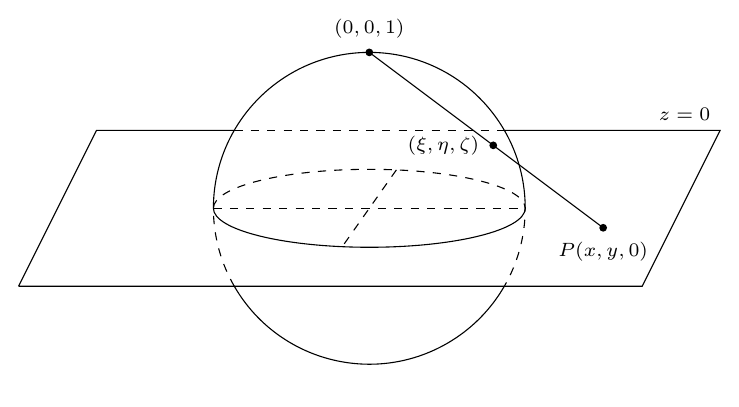
\includegraphics[width=0.90\textwidth]{stereographic_projection.png}
    \caption{Stereographic Projection Visualized}
\end{figure}
$$ v^{+} = S^2 \setminus \{(0,0,-1)\} \quad v^{-} = S^2 \setminus \{ (0,0,1) \} $$
We think of map $\phi^{-}$ as drawing a line through the point on the north pole $(0,0,1)$ and $(x,y,z)$, then the output is the point where the line intersects $z$ plane.
Similarly for $\phi^{+}$, we project from the south pole $(0,0,-1)$. We get the maps explicitly by parametrizing the line:
$$ l: (0,0,1) + t ((x_1,x_2,x_3) - (0,0,1)) =  (x_1 t,x_2 t, x_3 t-t+1) $$
$l$ intersects $x_3=0$ when $x_3t-t+1=$, thus $t = \frac{1}{(1-x_3)}$ It follows that the point of intersection is $(\frac{x_1}{1-x_3},\frac{x_2}{1-x_3},0)$
Similarly we can explicitly find $\phi^{+}$
$$ \phi_{+}: v^{+} \to \RR^2, \quad (x_1,x_2,x_3) \to (\frac{x_1}{1+x_3}, \frac{x_2}{1+x_3} )$$
$$ \phi_{-}: v^{-} \to \RR^2, \quad (x_1,x_2,x_3) \to (\frac{x_1}{1-x_3}, \frac{x_2}{1-x_3} )$$
We can find the inverses in the similar way.
Consinder points on the $z=0$ plane in $\RR^3$ $(\alpha, \beta, 0)$. We parametrize the line through this point and north pole:
$$ l: (0,0,1) + t((\alpha, \beta, 0 ) - (0,0,1)) = (\alpha t, \beta t, -t +1)$$
We need to see when are these points going to be on the sphere , i.e.
$$ (\alpha t)^2  + (\beta t)^2 + (-t +1)^2 = 1 $$
$$ \alpha^2 t^2 + \beta^2 t^2 + t^2 - 2t + 1 = 1 $$
$$ t^2 (\alpha^2 + \beta^2 +1 - \frac{2}{t} ) = 0 $$
$$ \therefore t = \frac{2}{\alpha^2 + \beta^2 +1 } $$
$$ \phi_{+}^{-1}:
\RR^2 \to v^{+} 
\quad (\alpha, \beta)  \to
( \frac{2 \alpha}{1+\alpha^2+\beta^2},
  \frac{2 \beta}{1+\alpha^2+\beta^2},
  - \frac{\alpha^2+\beta^2-1}{\alpha^2+\beta^2+1})
$$
$$ \phi_{-}^{-1}:
\RR^2 \to v^{-}
\quad (\alpha,\beta) \to
( \frac{2\alpha}{1+\alpha^2+\beta^2}, 
\frac{2\beta}{1+\alpha^2+\beta^2}, 
 \frac{\alpha^2 + \beta^2 -1}{\alpha^2+\beta^2+1} )
$$
Since we explicitly found an inverse, the function is a bijection.
\newline
And it's easy to see that $\phi$ is continuous by lemma \ref{contLemma} (denom never zero)
Thus we equipped the sphere with the following atlas:
$$ A_2 = \{(v^{\pm},\phi_{\pm}) \} $$
We can check that the transition maps from $A_1$ to $A_2$ are smooth. \newline
First we check for $\varphi_3^{+} \circ \phi_{+}^{-1}$ where
$$ \varphi_3^{+}: S^2 \cap {x_3 > 0} = u_3^{+} \to D_1(0,0) \subset \RR^2 $$
$$ \phi_{+}^{-1}: \RR^2 \to v^{+} = S^2 \setminus \{ (0,0,-1) \} $$
Now, since we require that the domain of $\varphi_3^{+}$ is positive, the following is how our transition function will look like

$$\varphi_3^{+} \circ \phi_{+}^{-1}: D_1 (0,0) \to D_1(0,0), \quad \varphi_3^{+}( \phi_{+}^{-1}(x_1,x_2)) = (\frac{2x_1}{1+x_1^2+x_2^2}, \frac{2x_2}{1+x_1^2+x_2^2})$$

$$ \phi_{+}^{-1} \circ \varphi_3^{+}: D_1 (0,0) \to D_1(0,0), \quad  \phi_{+}(\varphi_3^{+}((x_1,x_2) )^{-1}) = (\frac{x_1}{1+\sqrt{1-x_1^2-x_2^2}}, \frac{x_1}{1+\sqrt{1-x_1^2-x_2^2}})$$
It is continuous componentwise and thus smooth.
Next, we list the domain and the image for the rest of transition maps.
$$\varphi_3^{-} \circ \phi_{+}^{-1}: \RR^2 \setminus \bar{D_1} (0,0) \to D_1(0,0) \setminus (0,0)$$
$$\varphi_2^{+} \circ \phi_{+}^{-1}: \RR^2 \cap \{ x_2 > 0 \} \to D_1 (0,0)$$
$$\varphi_1^{+} \circ \phi_{+}^{-1}: \RR^2 \cap \{ x_1 > 0 \} \to D_1 (0,0)$$
$$\varphi_2^{-} \circ \phi_{+}^{-1}: \RR^2 \cap \{ x_2 < 0 \} \to D_1 (0,0)$$
$$\varphi_1^{-} \circ \phi_{+}^{-1}: \RR^2 \cap \{ x_1 < 0 \} \to D_1 (0,0)$$
$$\varphi_3^{+} \circ \phi_{-}^{-1}: \RR^2 \setminus \bar{D_1} (0,0) \to D_1(0,0) \setminus (0,0)$$
$$\varphi_3^{-} \circ \phi_{-}^{-1}: D_1 (0,0) \to D_1(0,0) $$
$$\varphi_2^{+} \circ \phi_{+}^{-1}: \RR^2 \cap \{ x_2 > 0 \} \to D_1 (0,0)$$
$$\varphi_1^{+} \circ \phi_{+}^{-1}: \RR^2 \cap \{ x_1 > 0 \} \to D_1 (0,0)$$
$$\varphi_2^{-} \circ \phi_{+}^{-1}: \RR^2 \cap \{ x_2 < 0 \} \to D_1 (0,0)$$
$$\varphi_1^{-} \circ \phi_{+}^{-1}: \RR^2 \cap \{ x_1 < 0 \} \to D_1 (0,0)$$
Therefore, we proved that a sphere $S^2$ is a smooth manifold of dimension $2$.
\end{proof}



\section{$G(1,3)$ as quotient manifold} 
We define the compact Stiefel manifold as:
\begin{equation}
St(p,n) = \{ A \in Mat_{n \times p}(\RR) \; | \; rkA = p, \; A^T A = I_k \}
\end{equation}
But if we consider the following $St(1,3) = \{ A \in \RR^{3 \times 1} \; | \; rkA=1, \; A^T A = 1 \} = \{ A \in \RR^3 \; | \; A^T A = 1 \} = 
\{ (A_1, A_2, A_3) \in \RR^3 \; | \; A_1^2 + A_2^2 + A_3^2 = 1) \} $ 
we see that this is exactly the equation of the sphere from \ref{s2}. Thus, $S^2 \cong St(1,3)$.
Now we will introduce an equivalence relation $ \sim $.
$$ \forall A,B \in St(1,3) \; B \sim A \text{ if } \; \exists \; g \in \RR, s.t. \; B = A g $$
which will identify antipodal points on the sphere.
If we quotient the Stiefel manifold with this relation, we get a sphere with antipodal points identified, namely: 
$$ \equivclass{St(1,3)} = \{ (A_1, A_2, A_3) \; | A_3 \geq 0 \} \cup \{ (A_1, A_2, 0) \; | \; A_2 \geq 0) \cup \{ (A_1, 0, 0) \}  $$

As mentioned in the introduction we consider the Grassmannian as follows:
$G(p,n) = \{ $p-dimensional (vector) subspaces of $\RR^{n \times p} \}$.
So if we take a line through all the points on $\equivclass{St(1,3)}$ we get a set of all lines in $\RR^3$, which is defined as $G(1,3)$. 
Hence, we arrive to the conclusion that we can consider a sphere with it's antipodal points identified as a quotient manifold of Stiefel $\equivclass{St(1,3)} \cong G(1,3)$
\newline

\section{$G(1,3)$ as a set of projectors}\label{g13proj}
We can easily see that $G(1,3) \cong \RR\PP^2$.
Consider a set of projectors $X \subseteq Mat_{3 \times 3}(\RR)$,
$$ X = \{ M \mid M^T = M, \: M^2 = M,\: Tr M = 1 \}$$
If we describe the embedding from $\RR \PP^2$ to $X$, we will understand why we can consider a sphere with antipodal points identified as a set of projectors.
\begin{Prop}
    There is an embedding from $\RR \PP^2$ to $X \subseteq Mat_{3 \times 3}(\RR) \cong \RR^9$ 
\end{Prop}
\begin{proof}
We know that $X$ consists of matrices that are symmetric, idempotent and whose eigenvalues add up to one.
Spectral theorem tells us that a real symmetric matrix is diagonizable.
We can also show that the eigenvectors of symmetric matrices, with distinct eigenvalues, are orthogonal.
Indeed, let $x$ and $y$ be eigenvectors of a symmetric matrix $M$, with eigenvalues $\lambda$ and $\mu$, $\lambda \neq \mu$:
$$ \lambda \langle x,y \rangle = \langle \lambda x,  y \rangle = \langle M x, y \rangle = \langle x M^T, y \rangle = \langle x, M y \rangle = \langle x, \mu y \rangle = \mu \langle x, y \rangle  $$
Therefore $(\lambda - \mu) \langle x , y \rangle = 0$, since $\lambda$ and $\mu$ are distinct $xy$=0, thus orthogonal.
\noindent  Next, we can show that the eigenvalues of $M$ can be only $0$ and $1$.
Let $v$ be an eigenvector, of eigenvalue $\lambda$.
$$ M v = \lambda v $$
$$ M^2 v = M (\lambda v) = \lambda M (v) = \lambda^2 v $$
As $\bar{v} \neq 0$ $(\lambda^2 - \lambda) v = 0 \iff \lambda^2 - \lambda = 0$.
Then solving for $\lambda^2-\lambda = 0$, we get that $\lambda$ can only be $0$ or $1$.
Finally, the fact that $Tr(M)=1$ tells us that eigenvalues of $M$ are $0$,$0$ and $1$.
Therefore $\dim \ker M = 2$ and $ \dim Im(M) = 1 $. This is telling us that there is a whole plane,
that is sent to zero vector by $M$, and all vectors in the image are sitting on a line.
\newline
Thus, applying a matrix operator $M$ to a vector,
is equivalent to projecting a vector to a line in $R^3$.
So $M :R^3 \to R^3$ is the operator of orthogonal projection on the line $Im(M)$.
\newline
Now, let's explicitly define a map $\phi$, which to given line in $R^3$ assigns a corresponding matrix operator,
that will orthogonally project all the vectors in $R^3$ to that line.
$$ \phi: \RR \PP ^2 \to Mat_{3 \times 3}  \quad \phi([x:y:z]) \to A $$
To explicitly find $A$, note that we first need to find a unit vector along a line $[x:y:z] \in \RR \PP ^2$,
we can do that by normalizing coordinates. $n = \frac{1}{\sqrt{x^2 + y^2 + z^2}} [x,y,z]^T $.
Finally, to orthogonally project any $v \in R^3$ along $n$, we apply $(v n) n = v \; n \otimes n$. We can then define $\phi$ as follows:
$$ \phi([x:y:z])  = \frac{1}{\sqrt{x^2+y^2+z^2}^2} [x,y,z]^T \otimes [x,y,z] = \frac{1}{x^2 + y^2 + z^2} 
\begin{pmatrix}
x^2 & xy & xz \\
xy & y^2 & yz  \\
xz & yz & z^2
\end{pmatrix} $$
Now, we redefine $\phi: \RR \PP ^2 \to \RR^6$, because  $Mat_{3 \times 3} \supseteq Sym_{3 \times 3} \simeq \RR^6$.
\begin{defn}{Immersion}
Let $X$ and $Y$ be smooth manifolds, $\dim X =n $, $\dim Y = k$. Let $f : X \to Y$ be a smooth map.
We say that $f$ is a
\begin{itemize}
    \item submersion, if $df_p$ is surjective $\forall p \in X$
    \item immersion, if $df_p$ is injective $\forall p in X$ equivalently if $rank D_p f = \dim M, M=f(X)$
\end{itemize}
\end{defn}
\begin{defn}
    Let $f: X \to Y$ be a smooth map of smooth manifolds. We say that $f$ is an embedding if 
    \begin{itemize}
        \item f is an injective immersion
        \item X is homeomorphic to $f(X) \subset Y$ (equipped with the subspace topology)
    \end{itemize}
\end{defn}
Next, we argue that $\phi \RR \PP ^2 \to R^6$ is an embedding ($R^6$ because we are taking only non-symmetric lower triangular entries)
Namely, we will show that the following function is an embedding.
$$ \phi([x:y:z]) = \frac{1}{x^2+y^2+z^2} (x^2,xy, xz, y^2, yz, z^2) $$
First, we show that $\phi$ is well defined. Take two vectors $a$,$b \in [x:y:z]$ on the same line.
If $a$ is given by $a=[a_1,a_2,a_3]$ then $b = [k a_1, k a_2, k a_3]$ for $k \in \RR$. We need to show that 
$\phi([a]) = \phi([b])$.
$$\phi([a_1,a_2,a_3]) = \frac{(a_1^2, a_1a_2, a_2^2, a_2a_3, a_3^2)}{a_1^2+a_2^2+a_3^2}$$
$$\phi([ka,kb,kc]) = 
\frac{(k^2 a_1^2, k^2 a_1a_2, k^2 a_2^2, k^2 a_2a_3, k^2 a_3^2)}{k^2 a_1^2+ k^2 a_2^2+ k^2 a_3^2} 
=  \frac{ k^2 (a_1^2, a_1 a_2, a_2^2, a_2a_3, a_3^2) }{ k^2 (a_1^2+a_2^2+a_3^2)  }
= \frac{(a_1^2, a_1a_2, a_2^2, a_2a_3, a_3^2)}{a_1^2+a_2^2+a_3^2} $$
Now that we showed that $\phi$ is well-defined, we show that it is injective.

\noindent Assume that $\phi$ is not injective, then there are unit vectors $a = [a_1,a_2,a_3]$ and $b=[b_1,b_2,b_3]$ lying on different lines 
such that $\phi([a]) = \phi([b])$ 
In other words $a \in [x:y:z]$  and $b \in [x ':y ':z ']$
$$\phi([a_1,a_2,a_3]) = (a_1^2, a_1a_2, a_2^2, a_2a_3, a_3^2)$$
$$\phi([b_1,b_2,b_3]) = (b_1^2, b_1b_2, b_2^2, b_2b_3, b_3^2)$$
From $\phi([a_1,a_2,a_3]) = \phi([b_1,b_2,b_3])$ we have that $b_1 = \pm a_1$, $b_2 = \pm a_2$, $b_3 = \pm a_3$, and we know that all $b_i$ have the same sign.
Therefore  we either have $b = [a_1, a_2, a_3]$ or $b = [-a_1, -a_2,-a_3]$ which both lie on the line $[x:y:z]$. So we have that $b \in [x:y:z]$ which is a contradiction.
\newline
We proved that $\phi$ is injective, and we know that $\RR \PP ^2$ is compact, so we proceed to proving that $\phi$ is an immersion, 
once we have that we can claim that $\phi$ is an embedding.
\newline
\noindent We can use the definition with local charts to prove it. 
Consider the following charts and maps.
$$ u_0 =  \{ [x:y:z], x \neq 0 \} \simeq \RR^2  $$
$$ u_1 =  \{ [x:y:z], y \neq 0 \} \simeq \RR^2  $$
$$ u_2 = \{ [x:y:z], z \neq 0 \} \simeq \RR^2  $$
$$ \psi_0: RP^2 \to \RR^2, \quad
\psi_0([x:y:z]) = (\frac{y}{x}, \frac{z}{x}), \quad
\psi_0^{-1}(s,t) = [1:s,t]
$$
$$ \psi_1: RP^2 \to \RR^2, \quad
\psi_1([x:y:z]) = (\frac{x}{y}, \frac{z}{y}), \quad
\psi_1^{-1}(s,t) = [s:1:t]
$$
$$ \psi_2: RP^2 \to \RR^2, \quad
\psi_2([x:y:z]) = (\frac{x}{z}, \frac{y}{z}), \quad
\psi_2^{-1}(s,t) = [s:t:1]
$$
These local charts cover all the points in $\RR \PP ^2$, to prove that $\phi$ is an immersion
we need to show the following, for all $p \in R^2$
$$ rank(J(\phi \circ \psi_i^{-1}(s,t))) = 2 $$
for $i \in {1,2,3}$.
\newline
We check for $\psi_0$.
$$\phi \circ \psi_0^{-1}(s,t) = [1:s:t] \to (1,s,t,s^2,st,t^2) \frac{1}{1+s^2+t^2} $$
$$ J(\phi \circ \psi_0^{-1}(s,t)) = \frac{1}{(1+s^2+t^2)^2} 
\begin{pmatrix}
-2s & -2t \\
-s^2+t^2+1 & -2st \\
-2st & s^2-t^2+1 \\
2s (t^2+1) & -2 s^2 t \\
t (-s^2 + t^2 +1 ) & s (s^2 - t^2 + 1) \\
-2st^2 & 2t(s^2+1)
\end{pmatrix} 
$$
To see that the rank is always $2$ we can check the the determinant of minor  $\Delta_{4,6} = 4 s t (s^2 + t^2 + 1)$ which is only zero when $st=0$.
But when both $s =0$ and  $t=0$ equal to zero, the determinant of the minor $\Delta_{2,3} = 1$, and if $\Delta_{2,3}$ is zero only if $s=1$ and $t=0$ or $s=0$ and $t=1$. 
But when that is the case $\Delta_{1,5} \neq 0 $. In conclusion there will always be a $2 \times 2$ minor with non-zero determinant, which means that our matrix has rank $2$.
Similarly we can check that $rank J(\phi_i) = 2$
\end{proof}

\noindent We can conclude that $\phi$ is an immersion, and thus embedding to $\RR^9$ and diffeomorphism to $\RR^6$.

\section{Gradient and Hessian on the sphere}

Tangent space of the sphere is given by 
$$ T_x St(1,3) = \{ v \in \RR^3 \; | \; xu^T V = 0 \} $$
Normal space is given as
$$ NxSt(1,3) = \{ a X \; | \; a \in \RR \} $$
We take the metric:
$$ g_c(\Delta,\Delta) = \tr \Delta^T (I - \frac{1}{2} X X^T ) \Delta  $$
We pick $\nabla$ to be the Levi-Civita connetion.
\newline
Let $f$ be a function that we want to calculate the gradient of, on the sphere.
Consider $f$ as a restriction of a function defined on the higher space, i.e. $f$ is defined on a submanifold and $\bar{f}$ is defined on the whole manifold.
In our case, the submanifold is a sphere $S^2$ and the higher manifold is $\RR^3$
$f = \bar{f}|_{\mathcal{M}}$
Every vector $\Delta \in T_x \RR^3$ admits a decomposition $\Delta = P_{x}\Delta + P_{x}^{\perp} \Delta$ where 
$ P_x \Delta \in T_{x} \mathcal{M} $ and $P_{x}^{\perp} \Delta \in T_{x}^{\perp} \mathcal{M}$.
Then the gradient is defined as:
$$\nabla f (x) =  grad f(x) = P_{x} grad \bar{f} (x) $$
Using this identity, we can now realize Levi-Civita connection by:
$$ \nabla_{\eta} grad f = P_{x} D (grad f(x))[\eta] = Hess f(x) \eta $$
We take the following projection $P_x = (I - xx^T)$.
\chapter{Grassman Manifold}\label{GrassChapter}
\section{Grassmannian as a smooth manifold}
Let us write $G(p,n) = \{ $p-dimensional (vector) subspaces of $\RR^{n \times p} \}$. A hyperplane $V \subseteq \RR^{n \times p}$ is specified by $n \times p$ matrix $A=[\vec{a}_1,\vec{a}_2, \dots, \vec{a_p}] \in Mat_{n\times p}$ where 
$\{\vec{a}_1, \vec{a}_2, \dots , \vec{a}_p \}$ is a basis for V. I.e., given $A \in Mat_{n\times p}$, $\rk A = p$, we get a p-hyperplane $V \subseteq \RR^{n \times p}$ by $V= $span $\{\vec{a}_1,\vec{a}_2, \dots, \vec{a}_p \} $. Conversely, given any p-dim subspace $V\subseteq \RR^{n \times p}$, there is a $n \times p$
matrix A with $\rk(A)=p$, from which $V$ is obtained in the above way. Two matrices, $A$ and $B$, determine the same subspace $V \iff \exists g \in GL(p) $, such that $B = A g$. $GL(p)$ stands for general linear group of degree $p$ over real field.
\newline
We thus have the following setup. Let the set of all  2-frames be
$$ F(p,n) = \{ A \; | \;  rkA=p \} \subseteq Mat_{n \times p}(\RR)  \simeq \RR^{n \times p} $$
and consider on it the equivalence relation
$$ B \sim A \text{ if } \exists \; g \in GL(p), \text{ s.t. } B=Ag $$
We have described a bijection of sets
$$ \equivclass{F(p,n)} \simeq  G(p,n). $$ 
We will show that $G(p,n)$ is a manifold equipped with a natural smooth structure. To achieve that we need to prove that:
\begin{itemize}
    \item $G(p,n)$ has a countable base
    \item $G(p,n)$ is Hausdorff
    \item $G(p,n)$ is locally euclidean
\end{itemize}
\begin{Prop}
    $F(p,n)$ is an open subset of $\RR^{p \times n}$
\end{Prop}
\begin{Lemma}\label{matrank}
    The rank of an $m \times n$ matrix is $r \iff$ some $r \times r$ minor does not vanish,
    and every $(r+1) \times (r+1)$ minor vanishes.
\end{Lemma}
Since we know that for $M \in F(p,n)^\complement$, $\rk M <p$ lemma \ref{matrank} tells us all $p \times p$ minors
of an arbitary element $ A \in F(p,n)^\complement$ vanish. Let's denote the determinant of each minor of $A$ with $S_i, \; i\in (1,2, \dots ,  {n \choose p})$ 
Then consider a continuous map
$ \psi: Mat_{n \times p} \to \RR^{ n \choose p}, \quad \psi(M) \to (S_1,S_2, \dots, S_{n \choose p})$.
We can express $F(p,n)^\complement = \psi ^{-1} ( \vec{0} )$ because all minors vanish (det=0).
A point $ \vec{0} \in \RR^{n \choose p}$ is a closed set, and because continuity preserves the closedness, $F(p,n)^\complement$ is closed in $Mat_{n \times p}$,
an since its complement is closed, $F(p,n)$ is an open subset of $Mat_{n \times p}(\RR)$
\begin{Prop}
    $\sim$ is an open equivalence relation on $F(p,n)$
\end{Prop}
In other words we need to show that the map $\pi: F(p,n) \to \equivclass{F(p,n)}$ is an open map.
Then $\pi$ is a quotient map and is equipped with $\equivclass{F(p,m)}$ is equipped with quotient topology.
\newline
\begin{Lemma} \label{quotientTop}
    A subset of a quotient space is open if and only if its
    preimage under the canonical projection map is open in the original topological space.
\end{Lemma}
Let $U$ be an open in $F(p,n)$. Then for every $g \in GL(p)$ the set $U g = \{ x g | x \in U \}$ is an open subset of $F(p,n)$.
Therefore $\pi^{-1}\pi(U) = \displaystyle \bigcup_{g \in G} \; U g$ is an open in $F(p,n)$ because the union of open sets is open.
And by \ref{quotientTop} $\pi(U) = [U]$ is open in $G(p,n)$. $\pi$ is a canonical quotient map, and $\equivclass{F(p,n)}$ is open in $\RR^{n \times p}$. 
\begin{Lemma}
    \label{baset}
    if $\beta = \{ \beta_\alpha \}_\alpha$ is a base for a topology $\mathcal{T}$ on a topological space $S$,
    and if $f: S \to X$ is an open map, then the collection $\{ f (\beta_\alpha) \}_\alpha$ is a base for the topology on $X$.
\end{Lemma}
\begin{proof} Let $V$ be an open in $X$ and $y \in V$. Choose $x \in f^{-1}(y)$. 
Since $f^{-1} (V)$ is open there is a basis element $U \in \beta$ s.t. $x \in U \subset f^{-1}(V)$
which implies that $y \in f(U) \subset V$. Since $y$ is arbitary, and $f(U) \subset f(\beta)$ the collection $\{ f (\beta_\alpha) \}_\alpha$ is a base for the topology on $X$.
\end{proof}
\begin{Prop}\label{secondCount}
    $G(p,n)$ has a second countable base.
\end{Prop}
\begin{proof}
We know that $F(p,n)$ has a second countable base since it is a subspace of $\RR^{n \times p}$.
Thus by lemma \ref{baset}, we have that the base of $G(p,n)$ is second countable.
\end{proof}
\begin{Prop}
The graph of the equivalence relation on $F(p,n)$ is a closed subset of $F(p,n) \times F(p,n)$. i.e. $ R = \{ (A,B) \in F(p,n) \times F(p,n) \; | \; A = Bg \}$ is closed.
\end{Prop}
\begin{proof}
We can consider $R$ as a set of matrices $[A B] = [\vec{a}_1, \vec{a}_2, \dots, \vec{a}_p, \vec{b}_1, \vec{b}_2, \dots , \vec{b}_p]$ of rank $p$.
Lemma \ref{matrank} tells us that every $(p+1) \times (p+1) $ minor of an element in $R$ must vanish. Consider the map that assigns to $(A,B)$ the values of all $ (p+1) \times (p+1) $ minors
$$ \psi:  F(p,n) \times F(p,n) \to \RR^{ {n \choose 3} (p+2) }$$
Since $\phi$ is continuous ( as all of its components are polynomials )  and $R = \psi^{-1} (0) $ , then R is closed.
\end{proof}
\begin{Ex}
    For example take $G(2,4)$, then $\phi: Mat_{4 \times 2} \to \RR^{16}$ 
\end{Ex}
\begin{Prop}\label{HausP}
$G(p,n)$ is Hausdorff.
\end{Prop}
\begin{proof}
Because $R$ is closed in $F(p,n) \times F(p,n)$, $(F(p,n) \times F(p,n)) \setminus R = R^{\complement}$ is open.
$\implies \forall (x,y) \in R^{\complement} $ there is a basic open set $u \times v$ containing $(x,y)$ s.t. $ (u \times v) \cap R = \emptyset 
\implies \forall x, y \text{ s.t. } (x,y) \not\in R, \exists$ u around x and v around y s.t. $u \cap v = \emptyset$
Thus for any two points $[x] \neq [y] \in \equivclass{F(p,n)}$ there exist disjoint neighborhood of $x$ and $y$ and $ \equivclass{F(2,4)}$ which is exactly the definition of Hausdorff property.
\end{proof}
\begin{Prop}\label{locEc}
   $G(p,n)$ is locally euclidean. 
\end{Prop}
\begin{proof}
Now that we have Hausdorff property and secound countable basis, we need to prove that every point lying on a manifold has a neighbourhood that is homeomorphic to an open in $\RR^n$.
Then we can claim that $G(p,n)$ is a manifold.
\newline
First we define charts. Take $A \in Mat_{n \times p} $ denote by $A_{k}$, ($ k \in \text{ all possible picks of p from the set } [1, \dots , n] $) the $p \times p$ minor, formed by the $k_1$th $\dots k_p$th rows of $A$.
The set
$$ U_{k} = \{ A \; | \; \det(A_{k}) \neq 0 \} \subset F(p,n)$$ is open, because its complement is closed. 
We also have that $\forall g \in GL(p)$ if $A \in U_{k}$ then $ Ag \in U_{k}$. 
Indeed, because $\det(Ag) = \det(A) \det(g)$, $\det( (Ag)_{i,j}) \neq 0$ which means $Ag$  will belong to a set $U_{k}$ 
Next, define
$$V_{k} = \equivclass{U_{k}} = \pi (U_{k}) \subset G(p,k)$$
The set $V_{k}$ is open since the equivalence relation is open. i.e. $\pi$ is an open map.
\newline
$U_k$ has a canonical representative $A \sim \widehat{A A_{k}^{-1}}$. $\widehat{\cdot}$ discards all the rows whose index is in $k$.
Similarly $V_k$ has a canonical representative: $[A] \sim [\widehat{A A_{k}^{-1}}] $

\begin{Ex}
Following the previous example consider $ [A] \in G(2,4)$.
If a minor $A_{2,4}$ is invertible we have that
$
[A] \sim [\widehat{A A_{2,4}^{-1}}] = 
\widehat{\begin{bmatrix}
* & * \\
1 & 0 \\
* & * \\
0 & 1
\end{bmatrix}} = \begin{bmatrix}  * & * \\ * & * \end{bmatrix}
$.
Since charts $ \bigcup U_k$ cover $F(p,n)$, charts $V_k$ cover $G(p,n)$ (because $\pi$ is open).
\end{Ex}
Now we define homeomorphisms between charts $V_k$ and opens in $R^{p \times (n-p)}$ as follows:
$$ \phi_{k}: V_{k} \subset G(p,n) \to Mat_{ (n-p) \times p} (\RR) \simeq \RR^{ (n-p) \times p) }, \quad \phi_{k}([A]) = \widehat{A A_{k}^{-1}} $$
We can show that $\phi$ is well defined. 
\newline
Let $A, A^\prime \in [A]$ we will show that $\phi$ is well defined. Equivalently $\phi_{k}(A) = \phi_{k}(A^\prime])$
Since $A$ and $A^\prime$ are in the same class, we have that $A^\prime = A g, \quad g \in GL(p) $, $\phi_{k}(A) = A A_{k}^{-1}$.
$$ \phi_{k}(A^\prime) = \phi_{k}(A g) = Ag ((Ag)_{k})^{-1} = Ag( A_{k} g )^{-1} = A g g^{-1} A_{k}^{-1} = A I A_{k}^{-1} = A A_{k}^{-1} = \phi_{k}(A) $$

$\phi$ is continuous because matrix multiplication is continous. Next, we can see that $\phi$ is surjective and $\phi^{-1}$ is continuous by explicitly defining inverse.

$$\phi_{k}^{-1}(\begin{pmatrix} \text{--- } \alpha_{1} \text{ ---}  \\ \vdots \\ \text{--- }  \alpha_{n-p} \text{ ---} \end{pmatrix}) =
\begin{pmatrix} 1_1 \\ \vdots  \\ 1_p \\ \alpha_1 \\ \vdots \\  \alpha_{n-p}  \end{pmatrix} $$
Finally, to show that $\phi$ is a homeomorphism,
we have left to shot that $\phi$ is injective. 
\newline
Assume that there $\phi_{k}$ is not injective then there are $A \in [A]$ and $B \in [B]$ such that there is \textbf{no} $g \in GL(p)$
for which $A g =  B$. i.e. $A A_{k}^{-1} = B B_{k}^{-1} \; \iff  \; 
 A A_{k}^{-1} B_{k} = B$ but $A_{k}^{-1} B_{k} \in GL(p)$ thus we reach contradiction.
Therefore $\phi_{k}$ is homeomorphism and we proved that $G(p,n)$ is locally Euclidean.
\end{proof}
\begin{Ex} \label{ex1}
    Let $A = \begin{bmatrix}
        2 & 6 \\
        1 & 3 \\
        2 & 1 \\
        4 & 3 \\
    \end{bmatrix}, \quad [ A ] \in V_{3,4}$
    $$ A A_{3,4}^{-1} =  \begin{pmatrix} 2 & 6 \\ 1 & 3 \\ 2 & 1 \\ 4 & 3 \\ \end{pmatrix} \begin{pmatrix} \frac{3}{2} & -\frac{1}{2} \\ -2 & 1 \\ \end{pmatrix}
    = \begin{pmatrix} -9 & 5 \\ -\frac{9}{2} & \frac{5}{2} \\ 1 & 0 \\ 0 & 1 \end{pmatrix}
    $$
    the above multiplication is continuous by \ref{quotientTop} and we can exlcude rows $3$ and $4$ so that we get result in $R^4$.
    Then the restriction to $R^4$ is also continuous.
    $$ \phi_{3,4}([A]) = \begin{pmatrix} -9 & 5 \\ -\frac{9}{2} & \frac{5}{2} \end{pmatrix} $$
\end{Ex}
Next the inverse map  $\phi_{3,4}(\beta)^{-1} \; \beta \in Mat_{2 \times 2} = \phi_{3,4}(A_{1,2} A_{3,4}^{-1} g) = [A] $ for some matrix $A$, such that $A_{1,2} = \beta$.
But if we pick $g = A_{3,4}$ then 
$ \phi_{3,4}(\beta) =
\begin{bmatrix}
    \beta_{1,1} & \beta_{1,2} \\ 
    \beta_{2,1} & \beta_{2,2} \\
    1 & 0 \\ 
    0 & 1 \\
\end{bmatrix}
$
More generally
$$\phi_{i,j}^{-1} : \RR^4 \to v_{i,j} \subset G(2,4) \quad \phi_{i,j}^{-1}(\beta) \to 
\begin{bmatrix}
    \beta \\
    I_{2 \times 2}
\end{bmatrix} = [\alpha]
$$
Such that $\alpha [i:] = \beta[1:]$, $\alpha[j:] = \beta[2:]$ , $\alpha[ (I \setminus \{i,j\})[1] ] = I[1:]$ and
$\alpha[ (I \setminus \{i,j \})[2] ] = I[2:]$
\newline
\begin{Ex}
   $ \phi_{3,4}^{-1} (\alpha) = [A] $ as defined in \ref{ex1}
   $$ \phi_{3,4}^{-1}  \begin{pmatrix} -9 & 5 \\ -\frac{9}{2} & \frac{5}{2} \end{pmatrix} = \begin{bmatrix} -9 & 5 \\ -\frac{9}{2} & \frac{5}{2} \\ 1 & 0 \\ 0 & 1 \end{bmatrix} $$ 
   We can confirm that $ \alpha = \begin{bmatrix} -9 & 5 \\ -\frac{9}{2} & \frac{5}{2} \\ 1 & 0 \\ 0 & 1 \end{bmatrix}$ and $A = \begin{bmatrix}
        2 & 6 \\
        1 & 3 \\
        2 & 1 \\
        4 & 3 \\
    \end{bmatrix}$
    span the same subspace.
    Because if we take $g = \begin{pmatrix} 2 & 1 \\ 4 & 3 \\ \end{pmatrix}$
    then $\alpha g = A$
\end{Ex}
Since $\bigcup U_{i,j}$ covers $F(2,4)$, $\cup v_{i,j}$ covers $G(2,4)$
Finally, we check transition maps.
$$ \phi_{1,2}([A])^{-1} = A_{3,4} A_{1,2}^{-1}, \quad \phi_{1,2}^{-1}(u) =
\begin{pmatrix}
1 & 0 \\
0 & 1 \\
v_{1,1} & v_{1,2} \\
v_{2,1} & v_{2,2}
\end{pmatrix}
$$

$$ \phi_{2,4}([A]) = A_{1,3} A_{2,4}^{-1}, \quad \phi_{2,4}^{-1}(v) = 
\begin{pmatrix}
v_{1,1} & v_{1,2} \\
1 & 0 \\
v_{2,1} & v_{2,2} \\
0 & 1
\end{pmatrix}
$$
$$ \phi_{2,4} \circ \phi_{1,2}^{-1}(v) = 
\begin{pmatrix}
v_{1,1} & v_{1,2} \\
v_{2,1} & v_{2,2}
\end{pmatrix} =
\begin{pmatrix}
    1 & 0 \\
    v_{1,1} & v_{1,2}
\end{pmatrix}
\begin{pmatrix}
    0 & 1 \\
    v_{2,1} & v_{2,2}
\end{pmatrix} ^{-1}
= 
\begin{pmatrix}
    1 & 0 \\
    v_{1,1} & v_{1,2}
\end{pmatrix}
\begin{pmatrix}
    v_{2,2} & -1 \\
    -v_{2,1} & 0
\end{pmatrix} \frac{1}{-v_{2,1}} = 
$$
$$ -\frac{1}{v_{2,1}} \begin{pmatrix} v_{2,2} & -1 \\ v_{1,1} v_{2,2} - v_{1,2} v_{2,1} & -v_{4} \end{pmatrix}
$$
\newline
Now let's check the transition map $ \phi_{3,4} \circ \phi_{2,3}^{-1} $ 
$$ \phi_{3,4} \circ \phi_{2,3}^{-1} (v) =
\begin{pmatrix} v_{1,1} &  v_{1,2} \\ 1 & 0 \end{pmatrix} 
\begin{pmatrix} 0 & 1 \\ v_{2,1} & v_{2,2} \end{pmatrix} = 
-\frac{1}{v_{2,1}} \begin{pmatrix} v_{1,1} v_{2,2} + v_{1,2} v_{2,1} & -v_{1,1} \\ v_{2,2} & -1 \end{pmatrix}
$$ 
\begin{Prop}
$G(p,n)$ can be equipped with the structure of a $p (n-p) $ dimensional smooth manifold.
\end{Prop}
The proof for the proposition follows from propositions \ref{locEc}, \ref{HausP}, \ref{secondCount},
and by checking that transition maps are infinitely differentiable.
\section{Grassmann manifold as a quotient manifold } \label{grassquot}
We will describe the Grassmann manifold as a quotient of the Stiefel manifold with respect to the orthogonal group.
\begin{center}
\begin{tikzcd}
St(p,n) \arrow[r, hook] \arrow[dr, dashrightarrow, "p"]
& F(p,n) \arrow[d, "\pi"]\\
& G(p,n)
\end{tikzcd}
\end{center}
Map $p$ is surjective because every subspace has an orthonormal basis.
I.e. starting with any basis we can construct an orthonormal one via Gram-Schmidt algorithm.
Now, if we redefine the map $p$ such that $p: { St(p,n) / _{O(p)}} \to G(p,n)$, where $O(p)$
is the orthogonal group of $2-frames$, we will have a bijection. 
To see why is it possible to quotient over $O(p)$ instead $GL(p)$ consider $A,B \in St(p,n)$ and consider that $A$ and $B$ are in the same subspace (go to the same point under equivalence relation) $A = B g, g \in GL(p)$.
We know that $ A^T A = I $, when we substitute we get $ (Bg)^T Bg = I \implies g^T B^T B g = I \implies g^T g = I$ which tells us that $g$ has to be an element of the orthogonal group.
Therefore 
$$ G(p,n) = F(p,n) / _{Gl_p(\RR)} \quad G(p,n) = St(p,n) / _{O(p) }$$
\section{Grassman manifold as a set of projectors }
Given
$$ X = \{ M \; | \; M^2 = M = M^T, trM=p \} \subset M_{n \times n} $$
We will prove that there is an embedding of $G(p,n)$ to $X$.
Based on the section \ref{g13proj} , we hypothesize that the embedding is given by
$$ \phi: \; G(p,n) \to X \quad \phi(A) = A(A^T A)^{-1} A^T  $$

\begin{Prop}
    $\phi$ is well defined
\end{Prop}
\begin{proof}
Take $A \in G(p,n)$ and $B \in G(p,n)$ s.t. $B = A g$. We know that $\phi(A) = A (A^T A)^{-1} A^T$ then
\begin{equation}
    \phi(B) = A g ((Ag)^T Ag)^{-1} (Ag)^{T} = A g (g^T A^T A g)^{-1} (A g)^{T} = A g g^{-1} (g^T A^T A)^{-1} g^T A^T = A (A^T A)^{-1} A^T
\end{equation}
\end{proof}
\begin{Prop}
    $\phi$ is injective
\end{Prop}
\begin{proof}
Assume that a function is not injective, then  $ \exists A, B \in G(p,n) \; $ s.t. $\phi(A) \neq = \phi(B) g$ for any $g$ in $GL(\RR)$ 
equivalently $A(A^T A)^{-1} A^T = B (B^T B)^{-1} B^T$, we use the fact that any $n \times p$ matrix $A$ can be decomposed as $A =  Q R$  where $Q$ is of shape $ p \times p$ and $R$ is of shape $n \times p$
then 
 $$ A(A^T A)^{-1} A^T =(QR) ((QR)^T QR)^{-1} (QR)^T = QR(R^T Q^T Q R)^{-1} R^T Q^T = $$
 $$ Q R (R^T R)^{-1} R^T Q^T = QRR^{-1} (R^T)^{-1} R^T Q^T = Q Q^T $$
But we know that there exists $Q$ such that $ \; \exists \; g$ s.t. $Q = Q'$. Therefore we get that $ A = Q R \quad B = Q' R'$ and $\phi(A) = Q Q^T = \phi(B) = Q' Q'^T$ but since $Q$ is orthogonal
we know that $ \; \exists \; g \; Q= Q' g \implies A = Bg$. we reach the contradiction and prove that $\phi$ is injective.
\end{proof}
\begin{Prop}
    $\phi$ is differentiable
\end{Prop}
\begin{proof}

$$\phi'(A) = (A (A^T A)^{-1} A)' = A' (A^T A)^{-1} A - A(A^T A)^{-1}(A' A^T) (A^T A)^{-1} A - $$
$$ A (A^T A)^{-1} (A (A^T)') (A^T A)^{-1} A^T + A (A^T A)^{-1} (A^T)'$$
Since we know that $A$ is differentiable this equation shows us that $\phi(A)$ is differentiable.

\end{proof}
\begin{Prop}
$P$ is a projection matrix to the subspace $A$, if given a vector $u$ that lies in the subspace, and $v$ that is perpendicular to the subspace $A$,
$Pu=u$ and $P v= 0$.
Show that $\phi(A)$ is a projector.
\end{Prop}
\begin{proof}
First we show that given a vector that already lies on $A$, the vector won't change.
Let $u = A v$, then $\phi(u) = A (A^T A)^{-1} A^T A v = A v = u$
Given a vector orthogonal to $A$ projection will go to zero. Take arbitary $u$ such that
$$ u = u^{\perp} + u^{\parallel} \quad u^{\parallel} \in Im A \; \implies \; u^{\parallel} = A v $$
Then $ u^{\perp} = u - u^{\parallel}$. Now to show that $\phi(u^{\perp}) = 0$
$$ \phi(u - u^{\parallel}) = \phi(u) - \phi(u^{\parallel}) = A (A^T A)^{-1} A^T u - A (A^T A)^{-1} A^T A v = Av - Av = 0 $$
We will in fact show that $X$ can be identified with $\equivclass{St(p,n)}$ which is (as we showed in \ref{grassquot} ) $G(p,n)$
\end{proof}
\begin{center}
\begin{tikzcd}
St(p,n) \arrow[r, hook] \arrow[dr, dashrightarrow, "p"]
& F(p,n) \arrow[d, "\pi"]\\
& G(p,n) \arrow[r, hook, "\phi"] 
& X
\end{tikzcd}
\end{center}
In this setup $A \in St(p,n)$ $\phi(A) = A(A^T A)^{-1} A^T = A A^T$
$$
D \phi (X) [V] = \lim_{t \to 0} \frac{ \phi( X + tV) - \phi(X) }{t} = 
\lim_{t \to 0} \frac{ (X + tV) (X + tV)^T - XX^T }{t} =
$$

$$
\lim_{t \to 0} \frac{ (X + tV) - (X^T + (tV)^T) - XX^T}{t} = \lim_{t \to 0} \frac{ XX^T X(tV)^T + tVX^T + tV(tV)^T - XX^T}{t} =
$$
$$
\lim_{t \to 0} \frac{ tXV^T + tVX^T + t^2 V V^T}{t} = XV^T + VX^T
$$
Take $V=\frac{1}{2} X B \quad B \in Sym(p)$
$$ \frac{1}{2} X A^T X^T + \frac{1}{2} X A X^T = X A X^T $$
It can be checked that $X A X^T \in X$ In other words for any matrix $X A X^T \in X$ there exists a matrix
$V \in \RR^{n \times p}$, such that $Dh(X)[V] = X A X^T$. 
Thus, $\phi$ is a defining function for $G(p,n)$ making it an embedded submanifold.
\section{Tangent Space}
To define a tangent and a normal space we need the metric.
When working on the Stiefel manifold the canonical metric is introduced with the purpose to restrict the orthogonal group metric to the horizontal space the canonical metric is introduced with the purpose to restrict the orthogonal group metric to the horizontal space.
Canonical metric on Stiefel is given as:
$$ g_c(\Delta_1, \Delta_2) = \tr \Delta ^T (I - \frac{1}{2} A A^T) \Delta 
$$
However the canonical metric on Grassman manifold is equivalent to the Euclidean metric
$$
g_c(\Delta_1, \Delta_2) = \tr \Delta_1^T (I - \frac{1}{2} Y Y^T) \Delta_2 = \tr \Delta_1^T \Delta_2 = g_e(\Delta_1,\Delta_2) 
$$
Thus we proceed with such choice of canonical metric.
\begin{Prop}
   The tangent space of $G(p,n)$ is given by all the commutators $ [ P, \Omega] = P \Omega - \Omega P \quad \Omega \in \mathfrak{so}_n  $ 
\end{Prop}
\begin{proof}
Consider the map $\delta: O(n) \to G(p,n), \quad \delta(T) = T P_0 T^T$. So that we fix $P_0$ to satisfy the following three conditions:
\begin{enumerate}
    \item $P^T = P \quad (T P_0 T^T)^T = T P_0^T T^T$
    \item $P^2 = P \quad (T P_0 T^T) (T P_0 T^T) = T P_0 T^T$
    \item $tr(T P_0 T^T) = tr (P_0 T^T T) = tr P_0 = k$
\end{enumerate}
Here these three rules are saying that we can get any projector $P_n = T P_0 T^T$
Note that $\delta$ is a submersion and therefore it induces a surjective map on tangent spaces.
The tangent space of $O(n)$ at the $n \times n$ identity matrix $I$ is
$ T_x O(n) = \{ \Omega \in \mathfrak{so}_n \} $ Note that $\Omega \in \mathfrak{so}_n$ means that omega is skew-symmetric $\Omega^T = -\Omega$.
Now if we take a derivative
$$ D_{\delta} : Tx O(n) \to T_{P_o} G(p,n), \quad \Omega \to P_0 \Omega - \Omega P_0 $$
\end{proof}
\begin{Ex}{ Tangent space in $G(1,3)$}
   Take $P = \begin{bmatrix} 1 & 0 & 0 \\ 0 & 0 & 0 \\ 0 & 0 & 0 \end{bmatrix} $
   find all $T_p X = \{ [P,\Omega] \; | \; \Omega \in \mathfrak{so}_n \}$
   $\Omega = \begin{bmatrix} \Omega_1 & -\Omega_2 & -\Omega_3 \\
                             \Omega_2 & \Omega_4 & -\Omega_5 \\
                             \Omega_3 & \Omega_5 & \Omega_6 \\ \end{bmatrix} $
    $\Omega P = \begin{bmatrix} \Omega_1 & 0 & 0 \\ \Omega_2 & 0 & 0 \\ \Omega_3 & 0 & 0 \end{bmatrix}$
    $ P \Omega = \begin{bmatrix} \Omega_1 & -\Omega_2 & - \Omega_3 \\ 0 & 0 & 0 \\ 0 & 0 & 0 \end{bmatrix} $
    Thus, the elements in the tangent spaces look like:
    $ P \Omega - \Omega P  = \begin{bmatrix} 0 & - \Omega_2 & - \Omega_3 \\ \Omega_2 & 0 & 0 \\ \Omega_3 & 0 & 0  \end{bmatrix}$
\end{Ex}
\begin{Ex}{Tangent space in $G(2,3)$}
   $P \in G(2,3) = \begin{bmatrix} 1 & 0 & 0 \\ 0 & 1 & 0 \\ 0 & 0 & 0  \end{bmatrix} $
   $ \Omega = \begin{bmatrix} \Omega_1 & -\Omega_2 & -\Omega_3 \\ \Omega_2 & \Omega_4 & -\Omega_5 \\ \Omega_3 & \Omega_5 & \Omega_6 \end{bmatrix}$
   $ P \Omega = \begin{bmatrix} \Omega_1 & - \Omega_2 & - \Omega_3 \\ \Omega_2 & \Omega_4 & - \Omega_5 \\ 0 & 0 & 0 \end{bmatrix}$
   $ \Omega P = \begin{bmatrix} \Omega_1 & - \Omega_2 & 0 \\ \Omega_2 & \Omega_4 & 0 \\ \Omega_3 & \Omega_5 & 0 \end{bmatrix}$
   Thus, the elements in the tangent space look like:
   $P \Omega - \Omega P = \begin{bmatrix} 0 & 0 & -\Omega_3 \\ 0 & 0 & -\Omega_5 \\ -\Omega_3 & - \Omega_5 & 0 \end{bmatrix} $
\end{Ex}
\begin{Ex}{Tangent space in $G(2,4)$}
    $P = \begin{bmatrix} 1 & 0 & 0 & 0 \\ 0 & 1 & 0 & 0 \\ 0 & 0 & 0 & 0 \\ 0 & 0 & 0 & 0 \end{bmatrix}$
    $\Omega = \begin{bmatrix} \Omega_1 & -\Omega_2 & -\Omega_3 & - \Omega_4 \\
                              \Omega_2 & \Omega_5 & - \Omega_6 & -\Omega_7 \\ 
                              \Omega_3 & \Omega_6 & \Omega_8 & - \Omega_9 \\ 
                              \Omega_4 & \Omega_7 & \Omega_9 & \Omega_{10}
                            \end{bmatrix}  $
    $P \Omega = \begin{bmatrix} \Omega_1 & -\Omega_2 & -\Omega_3 & -\Omega_4 \\
                            \Omega_2 & \Omega_5 & -\Omega_6 & -\Omega_7 \\
                            0 & 0 & 0 & 0 \\
                            0 & 0 & 0 & 0
                         \end{bmatrix} $
    $ \Omega P = \begin{bmatrix}
                \Omega_1 & -\Omega_2 & 0 & 0 \\
                \Omega_2 & \Omega_5 & 0 & 0 \\
                \Omega_3 & \Omega_6 & 0 & 0 \\
                \Omega_4 & \Omega_7 & 0 & 0 \\
                \end{bmatrix}$
    $ [P,\Omega] = \begin{bmatrix}
                0 & 0 & - \Omega_3 & -\Omega_4 \\
                0 & 0 & - \Omega_6 & - \Omega_7 \\
                - \Omega_3 & - \Omega_6 & 0 & 0 \\
                - \Omega_4 & - \Omega_7  & 0 & 0
    \end{bmatrix}
    $
\end{Ex}
Now, based on our examples, we can see that:
$ P_0 = \begin{bmatrix} I_p & 0 \\ 0 & 0 \end{bmatrix}$ where $I_p$ is $p \times p$ identity matrix.
For $G(p,n)$ we have the result $\begin{bmatrix} 0_p & A^T \\ A & 0_{n-p} \end{bmatrix}$
$\Omega = \begin{bmatrix} A & -B \\ B & C \end{bmatrix}$ where $A^T = -A$ and it's shape is $p \times p$ and $C^T = -C$ and it's shape is $(n-p) \times (n-p)$
$ P \Omega = \begin{bmatrix} A & - B^T \\ 0 & 0 \end{bmatrix} $
$ \Omega P = \begin{bmatrix} A & 0 \\ B & 0 \end{bmatrix}$
So the tangent space looks like:
$ [\Omega, P] = \begin{bmatrix} 0 & -B^T \\ B & 0 \end{bmatrix} $ where $B$ has the shape $ p \times (n-p) $
And because we considered this under equivalence relation $ Q \in O(p)$, the tangent of $G(p,n)$
is described as $T_x G(p,n) = \{ \Delta \; | \; \Delta = Q \begin{bmatrix} 0 & -B^T \\ B & 0 \end{bmatrix} \}$
\section{Normal Space}
$$ N_x G(p,n) = (T_x G(p,n))^{\perp} = \{ U \in \RR^{n \times p}: \langle U, V \rangle = 0 \text{ for all V } \in T_xG(n,p) \} $$
$$ N_x G(p,n = \{ U \in \RR^{n \times p} \; | \;  U^T  Q \begin{bmatrix} 0 & -B^T \\  B & 0 \end{bmatrix} = 0 \} ) $$ 
From here we can see that $U = Q \begin{bmatrix} A & 0 \\ 0 & C  \end{bmatrix} $
Therefore 
$$ N_x G(p,n) = \{ Q \begin{bmatrix} A & 0 \\ 0 & C  \end{bmatrix} \; | \;  Q \in O(p), A \in \mathfrak{so}(p), C \in \mathfrak{so}(n-p) \} $$ 
\section{Geodesic}
The orthogonal group geodesic is given as
$$Q(t) = Q(0) \exp t \begin{pmatrix} 0 & -B^T \\ B & 0 \end{pmatrix} $$
It has a horizontal tangent at every point along the curve $Q(t)$
$$ \dot{Q}(t) = Q(t) \begin{pmatrix} 0 & -B^T \\ B & 0 \end{pmatrix}$$
Thus Grassman geodesics = $ [ Q(t) ] $
The following theorem will be useful for computing the geodesic formula.
\begin{thm}
    If $Y(t) = Q e^{t \begin{pmatrix} 0 & -B^T \\ B & 0 \end{pmatrix} } I_{n,p} $ with $Y(0) = Y$ and $\dot{Y}(0) = H$, then
    $$ Y(t) = \begin{pmatrix} YV & U \end{pmatrix} \begin{pmatrix} \cos \Sigma t \\ sin \Sigma t \end{pmatrix} V^T $$
\end{thm}

\section{Parallel Transport}
\begin{thm}
    Let $H$ and $Delta$ be tangent vectors to the Grassmann manifold at $Y$.
    Then the parallel translation of $\Delta$ along the geodesic in the direction $\dot{Y}(0) - H$ is
    $$ \tau \Delta(t) = \begin{pmatrix} \begin{pmatrix} YV & U \end{pmatrix} \begin{pmatrix} -\sin \Sigma t \\ \cos \Sigma t \end{pmatrix} U^T + (I - UU^T) \end{pmatrix} \Delta $$
\end{thm}
\section{Gradient}
The gradient of $F$ at $[Y]$ is defined to be the tangent vector $\nabla F$ such that

\begin{equation}\label{gradEq}
    tr F_Y^{T} \Delta = g_c (\nabla F, \Delta) = tr(\nabla F)^T \Delta
\end{equation}
For all tangent vectors $\Delta$ at $Y$. \newline
Solving the equation \ref{gradEq} for $\nabla F$ such that $Y^T(\nabla F) = 0$ we get
\begin{equation}
    \nabla F = F_Y - Y Y^T F_Y
\end{equation}
\section{Hessian}
Hessian is defined as
$$ Hess F(\Delta_1, \Delta_2) = F_{YY}(\Delta_1, \Delta_2) - \tr(\Delta_1^T \Delta_2 Y^T F_Y) $$
For Newton's method, we must determine $\Delta = -Hess^{-1}G$, which for the Grassmann manifold is expressed as the linear problem:
$$ F_{YY}(\Delta) - \Delta(Y^T F_{Y}) = -G $$
\chapter{Optimization Algorithms}\label{OptChapter}
Classical Gradient Descent is defined as follows: 
\begin{enumerate}
\item $\Delta x_k = \frac{d}{d x_k} f(x_k) $
\item $x_{k+1} = x_{k} - lr \cdot \Delta x_k$
\end{enumerate}
It computed the gradient of the function, and then in the next steps move in the direction of gradient.
When the min/max is sufficiently close, it stops.
\newline
Newton's root finding method is given in the following two steps
\begin{enumerate}
    \item $\Delta x_k = - \frac{f(x_k)}{f'(x_k)}$
    \item $x_{k+1} = x_k + \Delta x_k$
\end{enumerate}
We perform optimization using Newton's method by applying it to the derivative of twice differentiable function $f$ to find the critical points.
\newline
Now we proceed by defining Gradient Descent and Newton's method on Grassmann manifolds.
We perform optimization with Newton's root-finding method by applying it to the derivative of the twice differentiable function $f$ to find the critical points.
\section{Gradient Descent}
Our objective is to minimize $F: G(p,n) \to \RR$. \newline
\begin{algorithm}
\caption{Gradient Descent method for minimizing $F(Y)$ on $G_1(p,n)$ }\label{alg:gradG}
    \begin{algorithmic}[1]
        \State \textcolor{red}{// Input: $F(\cdot)$ and the initial choice of $Y$ such that $Y^T Y = I_p$}
        \State \textcolor{red}{// Output: First $p$ columns of $Q$ whose span is the minimal subspace}
        \Procedure{MINIMIZE}{}
        \While{$||B|| < \epsilon$}\Comment{We define a stopping criteria}
        \State Compute the directional derivative $B$ and get the tangent $\Delta$
        \State
        \State Update $Q_{k+1} = Q_{k} \exp\{ \delta \Delta \} \text{ such that } f(U_{k+1}) > f(U_t)$
        \EndWhile
        \State \textbf{return} $Q[:,:p]$
        \EndProcedure
    \end{algorithmic}
\end{algorithm}
In the given algorithm $\delta$ stands for learning rate and $Q = \begin{pmatrix} U,V \end{pmatrix}$
\newpage
\section{Newton 1}
We have $F: G_1(p,n) \to \RR $, $ \; F(Y) = F(YQ), \; Y \in G_1(p,n), \; Q \in O(p), Y^T Y = I_p$
\begin{algorithm}
\caption{Newton's method for minimizing $F(Y)$ on $G_1(p,n)$ }\label{alg:quotAlg}
    \begin{algorithmic}[1]
        \State \textcolor{red}{// Input: $F(\cdot)$ and the initial choice of $Y$ such that $Y^T Y = I_p$}
        \State \textcolor{red}{// Output: $Y$ for which $F(Y)$ gives the minimum value}
        \Procedure{MINIMIZE}{}
        \While{$numSteps--$}\Comment{We have to choose the number of steps, or define some stopping criteria}
        \State $G = F_Y - Y Y^T F_Y$
        \State $\Delta = -Hess^{-1} G$ such that $Y^T \Delta = 0$ and $F_{YY}(\Delta) - \Delta(Y^T F_Y) = -G$
        \State
        \State Move from $Y$ in the direction $\Delta$ to $Y(1)$ using the formula 
        \State $Y(t) = Y V \cos(\Sigma t) V^T + U \sin(\sigma t) V^T$ \Comment{$U \Sigma V^T$ is SVD of $\Delta$}
        \EndWhile
        \State \textbf{return} $Y$
        \EndProcedure
    \end{algorithmic}
\end{algorithm}
\section{Newton 2}
For this one we define $F: Sym(n) \to \RR $ and  $f: G_2(p,n) \to \RR$ s.t. $f= F|_{G(p,n)}. \quad$
$ ad_p(X) = [P, X] = PX -  XP $
$M_Q$ subscript means that we are taking only $Q$ part from the $QR$ decomposition of $M$
\begin{algorithm}\label{newton2}
\caption{Newton's method for minimizing $F(M)$ on $G_2(p,n)$ }\label{alg:projAlg}
    \begin{algorithmic}[1]
        \State \textcolor{red}{// Input: $F(\cdot)$ and the initial choice of $M$ such that $M^T=M, M^2=M, TrM=p$}
        \State \textcolor{red}{// Output: $M$ for which $F(M)$ gives the minimum value}
        \Procedure{MINIMIZE}{}
        \While{$numSteps--$}\Comment{We have to choose the number of steps, or define some stopping criteria}
        \State Solve
        \State $ad^2_{M} Hess_{F}(M)(ad_{M}\Omega) - ad_{M} ad_{\nabla F (M) } ad_{M} \Omega = -ad^2_{M} \nabla_{F}(M)$
        \State for $\Omega \in skew_-sym(n) $
        \State
        \State Solve 
        \State $M = \Theta^T \begin{bmatrix} I_m & 0 \\ 0 & 0 \end{bmatrix} \Theta$ \Comment{$\Theta$ is orthonormal}
        \State for $ \Theta \in SO_n$
        \State
        \State $ M = \Theta^T (\Theta( I - ad^2_{M} \Omega ) \Theta^T)_Q     \Theta M \Theta^T    (\Theta (I - ad^2_{M} \Omega) \Theta^T)_Q^T    \Theta$
        \EndWhile
        \State \textbf{return} $M$
        \EndProcedure
    \end{algorithmic}
\end{algorithm}

\chapter{Minimize Rayleigh Quotient}\label{RayChapter}
The Rayleigh quotient for a given symmetric matrix $M$ and a nonzero vector $x$ is defined as
$$ R(M,x) = \frac{x^T M x}{x^T x}$$
\begin{thm}
    For any given symmetric matrix $M \in \RR^{n \times n}$
    $$ max_{x \in \RR^{n}: x \neq 0} \frac{x^T M x}{x^T x} \text{ (when x = "largest" eigenvector of M) } $$
    $$ min_{x \in \RR^{n}: x \neq 0} \frac{x^T M x}{x^T x} \text{ when x = "smallest" eigenvector of M } $$
    \begin{proof}        
        Let $M = Q \Lambda Q^T$ be the spectral decomposition, where $Q = [q_1, \dots, q_n]$ is orthogonal and 
        $\Lambda = diag(\lambda_1, \dots, \lambda_n) $ is diagonal with sorted diagonals from large to small.
        Then for any unit vector $x$,
        $$ x^T M x x^T (Q \Lambda Q^T) x = (x^T Q) \Lambda (Q^T x) = y^T \Lambda y $$
        where $y = Q^Tx$ is also a unit vector:
        $$ || y ||^2 = y^T y = (Q^T x)^T (Q^T x) = x^T Q Q^T x = x^T x = 1 $$
        So the original optimization problem becomes:
        $$ max_{y \in \RR^n : || y || =1 } y^T \Lambda y \textbf{ (Lambda diagonal)}  $$
        To solve this problem write $y = (y_1, \dots, y_n)^T$. It follows that:
        $$ y^T \Lambda y = \sum_{i=1}^{n} \lambda_i y_i^2  $$
        Because $\lambda_1 \geq \lambda_2 \geq \dots \lambda_n$, when
        $y_1^2 = 1, y_2^2 = \dots = y_n^2 = 0$
        the objective function attains its minimum value $y^T \Lambda y = \lambda_1$
        In terms of the original variable $x$, the maximizer is
        $$ x^{*} = Qy^{*} = Q (\pm e_q) = \pm q_1 $$
        In conclusion, when $x=\pm q_1$ (largest eigenvector), $x^TMx$ attaints its maximum value $\lambda_1$ (largest eigenvalue)
    \end{proof}
\end{thm}
In the next subsections we will focus on \textbf{Computing the eigenvectors and eigenvalues of a symmetric matrix by minimizing rayleigh quotient}
\section{Gradient Descent on the sphere}
We have the following setup: \newline
Compute $ min_{x \in S^n} \frac{1}{2} x^T M x $ \newline
The cost function $f: S^n \to \RR$ is the restriction of $\bar{f} = \frac{1}{2} x^T M x $ from $\RR^n to S^n$ \newline 
Tangent spaces are given by $T_x S^n = \{ v \in \RR^n : x^T v = 0 \}$ \newline
To make $S^n$ into a Riemmannian submanifold of $\RR^n$ we take a dot product $\langle u, v \rangle = u^T v $ 
Projection to $T_x S^n$: $Proj_x(z) = z - (x^T z)x$ \newline
Gradient of $\bar{f} = \nabla \bar{f} (x) = M x$ \newline
Gradient of $f$: $grad f(x) = Proj_x(\nabla \bar{f} (x)) = Mx - (x^T M x) x$
Thus algorithm becomes

\begin{algorithm}
\caption{Gradient Descent method for minimizing the Rayleigh quotient}
    \begin{algorithmic}[1]
        \State \textcolor{red}{// Input: The initial choice of $Y$ such that $Y^T Y = I_p$ and the choice of learning rate $lr$}
        \State \textcolor{red}{// Output: $Y$ for which of $F(Y)$ gives the dominant eigenvalue}
        \Procedure{MINIMIZE}{}
        \For{$i$ in $num_{.}steps$}\Comment{Define a number of steps or a stopping criteria}
        \State if $i \mod 100 == 0$ then $lr = lr/100$ \Comment{Learning rate decay}
        \State $Y = Y - lr \cdot  \nabla f (X)$
        \EndFor
        \State \textbf{return} $Y$
        \EndProcedure
    \end{algorithmic}
\end{algorithm}
\begin{Ex}
    Find the dominant eigenvector and eigenvalue of $A = \begin{pmatrix} 181 & 101 & 146 \\ 101 & 74 & 103 \\ 146 & 103 & 146 \end{pmatrix} $ 
    by using gradient decent on Rayleigh quotient.
\end{Ex}
\begin{figure}[h] \label{gradRay}
    \centering
    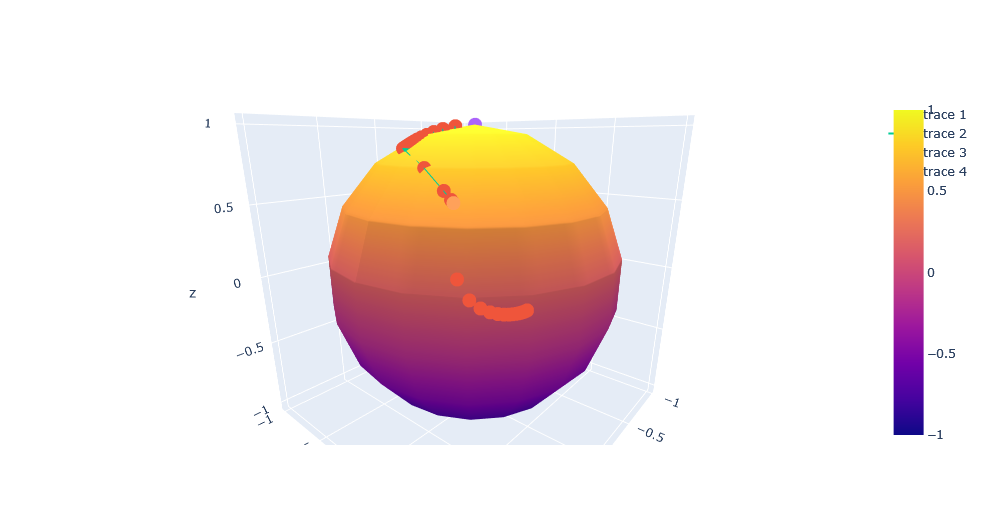
\includegraphics[width=0.90\textwidth]{gradientDescent1.png}
    \caption{Convergence of the GD algorithm on Rayleigh quotient example}
\end{figure}
\newpage
\section{Newton 1}
Given the function $\bar{f}= x^T M x \quad grad \bar{f} = 2 M x  - 2 (x^T M x) = 2 (I - xx^T) A x = 2 P M x$
$$ D(grad f) = 2M - 4 x M x \eta + 2 x^T M x $$
Reminder $g_c(\Delta,\Delta) = tr \Delta^T (I - \frac{1}{2} Y Y^T) \Delta$
$$ g_c (D(grad f), \eta ) = g_c(2M - 2x^T M x + 4M x x^T, \eta) = 2 M  P \eta  - 2 \eta x^T M x  $$
$$ P g_c(D(grad f), \eta) = 2 M P \eta - 2 \eta x^T M x$$
Therefore we have a Newton iteration:
$$ P_x M P_x \eta - \eta x M x = - P M x$$
\begin{algorithm}
\caption{Newton's method for minimizing the Rayleigh quotient}
    \begin{algorithmic}[1]
        \State \textcolor{red}{// Input: The initial choice of $Y$ such that $Y^T Y = I_p$}
        \State \textcolor{red}{// Output: $Y$ for which $F(Y)$ gives the minimum value}
        \Procedure{MINIMIZE}{}
        \While{$numSteps--$}\Comment{ define some stopping criteria}
        \State $M = P(Y) M P(Y) - x^T A x $
        \State $y = - P(Y) A x$
        \State $\eta = solve(M,y)$
        \State $Y = R(Y, \eta)$
        \EndWhile
        \State \textbf{return} $Y$
        \EndProcedure
    \end{algorithmic}
\end{algorithm}
$P$ is a projection, $R$ is a retraction.
\begin{Ex}
    Find eigenvectors and eigenvalues of $A = \begin{pmatrix} 181 & 101 & 146 \\ 101 & 74 & 103 \\ 146 & 103 & 146 \end{pmatrix} $ using Newton 1
\end{Ex}
OUTPUT: $ [-0.74148822,  0.44835462,  0.49917267] $
\begin{figure}[h] \label{gradR1}
    \centering
    \includegraphics[width=0.90\textwidth]{newton1.png}
    \caption{Convergence of the Newton 1 algorithm on Rayleigh quotient example}
\end{figure}

\section{Newton 2}

For the Rayleigh quotient the equation that we need to solve in the first step of \ref{newton2} becomes:
$$ -ad_{P_j} ad_{A} ad_{P_j} \Omega_j = - ad^2_{P_j} A = \Theta_j(ad_{P_j} ad_A ad_{P_j} \Omega_j) \Theta_j^T = \Theta_j (ad_{P_j}^2 A) \Theta_j^T  $$
%and using
$$ P_j = \Theta_j^T \begin{bmatrix} I_m & 0 \\ 0 & 0 \end{bmatrix} \Theta_j $$
%is the same as solving
$$ ad_{\begin{bmatrix} I_m & 0 \\ 0 & 0  \end{bmatrix} } ad_{\Theta_j A \Theta_j^T} ad_{\begin{bmatrix} I_m & 0 \\ 0 & 0 \end{bmatrix}}
    \begin{bmatrix} 0 & Z_j \\ -Z_j^T & 0 \end{bmatrix} = ad^2_{\begin{bmatrix}  I_m & 0 \\ 0 & 0 \end{bmatrix}} (\Theta_j A \Theta_j^T)$$ 
    for $Z_j \in \RR^{m \times (n-m)}$. Denoting
    $$\Theta_j A \Theta_j^T = \begin{bmatrix} A_{11} & A_{12} \\ A_{12}^T & A_{22} \end{bmatrix} $$
    so we just have to solve the Sylvester equation
    $$ A_{11} Z_j - Z_j A22 = A_{12} $$

\begin{algorithm}
\caption{Newton's method for minimizing Rayleigh quotient on $G_2(1,3)$ }
    \begin{algorithmic}[1]
        \State \textcolor{red}{// The initial choice of $\Theta \in SO(n)$}
        \State \textcolor{red}{// Output: $\Theta$ whose first $p$ are the eigenvector}
        \Procedure{MINIMIZE}{}
        \While{$numSteps--$}\Comment{define some stopping criteria}
        \State Compute $\begin{bmatrix} A_{11} & A_{12} \\ A_{12}^T & A_{22} \end{bmatrix} = \Theta_j A \Theta_j^T$
        \State Solve the Sylverster equation $A_{11} Z_j - Z_j A_{22} = A_{12}$ for $Z_j \in \RR^{m \times (n-m)}$
        \State 
        \State Compute $\Theta_{j+1}^T = \Theta_j^T \begin{bmatrix} I_m & Z_j \\ -Z_j^T & I_{n-m} \end{bmatrix}_Q $ 
        and 
        $ P_{j+1} = \Theta_{j+1}^T \begin{bmatrix} I_m & 0 \\ 0 & 0 \end{bmatrix} \Theta_{j+1} $
        \EndWhile
        \State \textbf{return} $M$
        \EndProcedure
    \end{algorithmic}
\end{algorithm}
\begin{Ex}
    Find eigenvectors and eigenvalues of $A = \begin{pmatrix} 181 & 101 & 146 \\ 101 & 74 & 103 \\ 146 & 103 & 146 \end{pmatrix} $ using Newton 2
\end{Ex}
OUTPUT: $ [-0.74364137,  0.43442584,  0.5082044 ]$
\begin{figure}[h] \label{gradR2}
    \centering
    \includegraphics[width=0.90\textwidth]{newton2.png}
    \caption{Convergence of the Newton 2 algorithm on Rayleigh quotient example}
\end{figure}

\chapter{Notation}  
\noindent\begin{tabularx}{\textwidth}{@{}XXX@{}}  \toprule
  Symbol & Matrix Definition & Name \\
  \toprule
  $F(p,n)$  & $\{A \in Mat_{n \times p}  \; | \; rkA = p  \} $ & 2 frames \\
  \toprule
  $St(p,n)$ & $ \{ A \in F(2,4) \; | \; A^T A = I_k \} $ & Stiefel Manifold \\
  \toprule
  $ GL(p)$ &  $ \{ A \in Mat_{n \times n} \; | \; det A \neq 0 \}$ & General Linear Group \\
  \toprule
  $ O(p)$ & $ \{ Q \in GL(p) \; | \; Q^T Q = I \}$  & Orthogonal group \\
  \toprule
  $ \mathfrak{so}_n $ & $ \{ \Omega \in \RR^{n \times n} \; | \; \Omega^T = - \Omega \} $ & Real skew-symmetric matrices \\
  \toprule
  $ Sym(p) $ & $ \{ A \in \RR^{p \times p} \; | \; A^T = A \} $ & Symmetric matrices \\
  \toprule
  $ SO(n) $ & $ \{ Q \in O(n) \; | \; \det(Q) = 1 \} $ & Special Orthogonal Group \\
\end{tabularx}\offinterlineskip

 
\bibliographystyle{alpha}
\bibliography{biblio}
 %%% STIEFEL NORMAL SPACE %%%%%%%%%
%Consider $h: \RR^{n times p} \to Sym(p) \quad X \to h(x) = X^T X - I_p$
%Sym is a manifold of dimension $k = \frac{p (p+1)}{2}$, $h$ is smooth and $h^{-1}(0) = St(p,n)$, so $h$ is a defining function for $St(p,n)$
%We show that $0$ is a regular value, if for all $p \in h^{-1}(0)$ the differential $D h_p: T_p \RR^{n \times p} \to T_{h(x)} Sym P$
%is a surjetive function. And it's surjective if the differential has rank $k$.
%$Dh(X): \RR^{n \times p} \to Sym(p) \quad Dh(X)[V] =  \lim_{t \to 0} \frac{h (X + tV) - h(X)}{t} =
%\lim_{t \to 0} \frac{(X + tV)^T (X+tV) - X^T X}{t} = X^TV + V^T X $
%If we perform polar decomposition we get that $V= \frac{1}{2} XA \quad A \in Sym(p)$
%\newline
%$Dh(X)[V] = \frac{1}{2} X^T X A + \frac{1}{2} A^T X^T X = A$ thus the image of $Dh(X)$ is all of $Sym(p)$ so it has rank $k$.
%So $St(p,n)$ is emedded in $\RR^{n times p}$ and $dim St(p,n) = dim \RR^{n times p} - dim Sym(p) = np - \frac{p (p+1)}{2}$
%$TxSt(p,n) = ker Dh(x) = \{ V \in \RR^{n times p} : X^T V + V^T X = 0 \} $
%Pick $X_{\perp}$ such that
%$$ X^T X = I_p \quad X_{\perp}^T X_{\perp} = I_{n-p} \quad X^T X_{\perp} = 0 $$ 
%Then $V = \begin{bmatrix} X & X_{\perp} \end{bmatrix} \begin{bmatrix} \Omega \\ B \end{bmatrix}$ where $\Omega \in \mathfrak{so}(p) \quad B \in \RR^{ (n-p) \times p} $
%We arrive to the following definition of the tangent space to Stiefel:
%$$ T_x St(p,n) = \{ X \Omega + X_{\perp} B \; | \; \Omega \in \mathfrak{so}(p), B \in \RR^{ (n-p) \times p} \} $$
%Now we proceed on defining a normal space to Stiefel.
%$$ N_x St(p,n) = (T_x St(p,n))^{\perp} = \{ U \in \RR^{n \times p}: \langle U, V \rangle = 0 \text{ for all V } \in TxSt(n,p) \} $$ 
%$$ N_x St(p,n) = \{ U \in \RR^{n \times p} : \langle U, X\Omega + X_{\perp} B \rangle = 0$$
%Expand $U = AX + X_{\perp} C, A \in \RR^{p \times p, C \in \RR^{ (n-p) \times p}}$
%$$ NxSt(p,n) = \{ U \in \RR^{n \times p} : \langle XA + X_{\perp} C, X \Omega + X_{\perp} B \rangle = 0$$
%$$ NxSt(p,n) = \{ U \in \RR^{n \times p} : \langle A, \Omega \rangle = 0 and \langle C, B \rangle = 0 \} = \{ XA \; | \; A\in Sym(p) \}$$
%\newline
%$$ U - Proj_{x} (U) = XA$$
%$$ Proj_{x}(U)^T X + X^T Proj_{x} (U) = 0 $$
%$$ (U - XA) ^T X + X^T (U- XA ) = 0$$
%$$ U^T X - A + X^T U - A = 0$$
%$$ U^T X + X^T U = 2A $$
%$$ Proj_{X} (U) = U - X \frac{X^T U + U^T X}{2} = (I - XX^T)U + X \frac{X^T U - U^T X}{2} $$
\end{document}          
